%!TEX root = ../TAMUTemplate.tex
%%%%%%%%%%%%%%%%%%%%%%%%%%%%%%%%%%%%%%%%%%%%%%%%%%%
%
%  New template code for TAMU Theses and Dissertations starting Fall 2016.
%
%  Author: Sean Zachary Roberson
%    Version 3.16.09
%  Last updated 9/12/2016
%
%%%%%%%%%%%%%%%%%%%%%%%%%%%%%%%%%%%%%%%%%%%%%%%%%%%
%%%%%%%%%%%%%%%%%%%%%%%%%%%%%%%%%%%%%%%%%%%%%%%%%%%%%%%%%%%%%%%%%%%%%%
%%                           SECTION IV
%%%%%%%%%%%%%%%%%%%%%%%%%%%%%%%%%%%%%%%%%%%%%%%%%%%%%%%%%%%%%%%%%%%%%



\chapter{\uppercase {Event Reconstruction}}
\label{ch:event_reconstruction}

The CMS detector is designed to identify the various particle species which travel through it after a proton-proton collision.
As discussed in chapter~\ref{ch:LHC_CMS}, the sub-detector technologies were chosen so that particles could be identified by where they deposit their energy as well as how their trajectories change in a magnetic field.
Fig.~\ref{fig:particle_flow} shows how various types of particles interact with the CMS detector.
All of the charged particles (\ie electrons, muons, and charged hadrons) will deposit some energy in the tracker, while neutral particles (\ie photons and neutral hadrons) will not.
Electrons and photons will deposit all of their energy inside of the ECAL while hadrons, both charged and neutral, will deposit most of their energy in the HCAL.
Muons are the only visible particle which will be able to travel to the muon chambers.
Neutrinos will pass through all layers of the detector unseen and their presence must be inferred by missing transverse energy (\MET or \ETslash); the idea being that if the sum of the transverse momentum is not conserved, then that missing momentum must correspond to at least one unseen particle.

\begin{figure}[!hbt]
    \centering
    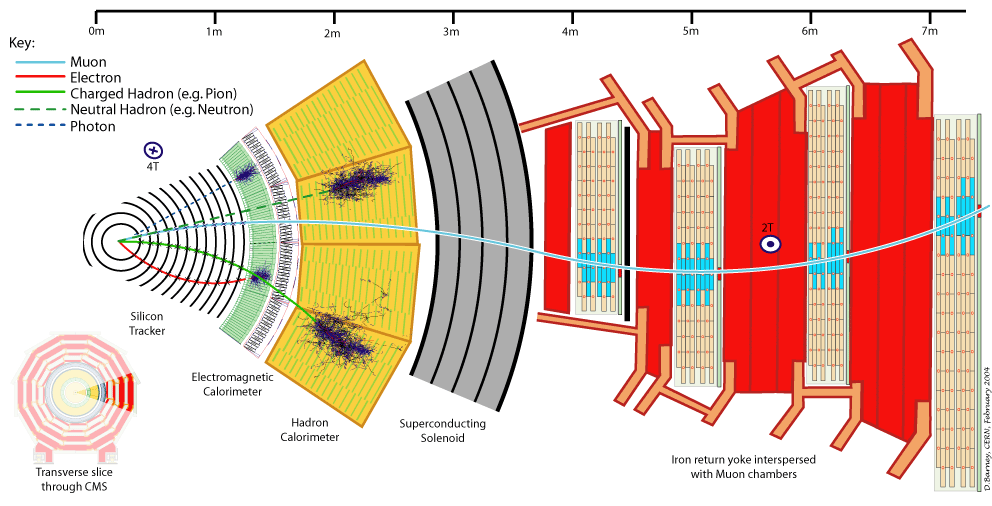
\includegraphics[width=0.95\textwidth]{\figpath/Chapter3/ParticleFlow}
    \caption{Cross-sectional view of the CMS detector with all of the sub-detectors labeled.The colored lines correspond to different particle species, which interact with different pieces of the detector and may or may not be bent by the magnetic field.}
    \label{fig:particle_flow}
\end{figure}
t
The process of translating abstract detector objects to physical particles takes several steps within the CMS software framework (CMSSW).
The first of this process is local reconstruction, where the various subsystems of each sub-detector create what are called reconstructed hits, or RecHits for short.
RecHits in the tracker contain information about the position of energy clusters (groups of contiguous strips or pixels which contain a signal) as well as energy deposition information which aids in particle identification.
The muon RecHits ostensibly contain information about the position of the signal.
However, the RecHits from the DTs and CSCs can be combined to form three-dimensional track segments, which also provide directional information.
The ECAL and HCAL RecHits contain information about the energy deposited, the position of those deposits, and the time at which they occurred.

The next step is to process this information in a global manner, where the subsystems within each sub-detector are combined.
Pattern recognition algorithms are run on the tracker RecHits to reconstruct the path that the particles take through the sub-detector (a.k.a tracks).
The ECAL and HCAL RecHits within a tower are summed to form ``CaloTowers'' which have a projective $\eta-\varphi$ geometry.
The muon system creates ``standalone'' muons by associating RecHits and track segments with compatible radial trajectories.
This process takes into account the bending a muon undergoes before reaching and within the muon system due to the magnetic field.

At this point, all of the reconstruction information is combined to form particles that can be used for physics analysis.
The process of reconstructing and classifying every stable particle is called Particle Flow (PF) and will be discussed further in chapter~\ref{sec:particle_flow}.
This analysis focuses on electrons, muons, jets, b-jets, and \ETslash, the reconstruction of which will be described in the following sections.
Additional information about the reconstruction process beyond the scope of this thesis can be found in~\cite{TDR-software}.

\section{Tracks and Vertices}
\label{sec:tracks_and_vertices}

While CMS analyses cover a wide range of final states, a majority of them will include jets in some fashion, including this one.
It's important that the particle flow algorithm identify and measure each particle inside a jet in order to improve the jet energy response and resolution.
Section~\ref{sec:jets} will cover the reconstruction and properties of jets in more detail, but it is important to note that two thirds of the constituents inside of a jet are charged particles.
This motivates the need for excellent tracking capabilities.
Tracks are created from the RecHits using the Combinatorial Track Finder (CTF) algorithm, which is an iterative process~\cite{TRK-11-001}.
This process seeks to find the appropriate balance between high reconstruction efficiency and low fake rate (see fig.~\ref{fig:efficiency_vs_fake_rate})~\cite{CMS-PAS-PFT-09-001}.

\begin{figure}[!hbt]
    \centering
    \begin{tikzpicture}[node distance = 2cm, auto]
        \tikzstyle{myarrows}=[line width=1mm,-triangle 45,postaction={draw, line width=3mm, shorten >=4mm, -}]
    
        \node (up) at (0,2) {};
        \node (center) at (0,0) {};
        \node (down) at (0,-2) {};
    
        \draw[myarrows,green!50!black] (center) -- node[right,black,xshift=5mm] {Reconstruction Efficiency} ++ (up);
        \draw[myarrows,red] (center) -- node[right,black,xshift=5mm] {Fake Rate} ++ (down);
    
        \node (smiley) at (-1,1)  {\Smiley[3][green!50!black]};
        \node (sadey)  at (-1,-1) {\Sadey[3][red]};
    \end{tikzpicture}
    \caption{A diagram showing the goals of the iterative tracking process.}
    \label{fig:efficiency_vs_fake_rate}
\end{figure}

The track finding procedure begins by finding track seeds using only a few hits and very tight criteria.
A track is built by extrapolating from the trajectory of the seed and adding new hits that match this trajectory, keeping in mind that charged particles will bend in the presence of the magnetic field.
The tight requirements on this first step lead to a moderate tracking efficiency and a vanishingly small fake rate.
After a track is found, all of the hits are used in a fit to determine the track parameters (i.e. \pt, $\chi^{2}$, etc.), which are then used to judge the quality of the track.
If a track doesn't meet certain quality requirements on the \pt, the transverse impact parameter $d_{0}$, and the longitudinal impact parameter $d_{z}$, it isn't kept.
Additionally, a trajectory cleaning step to remove duplicate tracks is applied to each iteration and to the final track collection.
A duplicate track can form either from different seeds or from the same seed which forms two very similar tracks.
If a pair of any two tracks share more than 19\% of hits as determined by equation~\ref{eq:trajectory_cleaning}, where $N^{hits}_{1}$ and $N^{hits}_{2}$ are the number of hits used in forming the tracks and 19\% is an empirically determined value, then the track with the fewest number of hits or the largest $\chi^{2}$ is removed.
The hits which are unambiguously assigned to the tracks are removed from consideration in the next iteration and their tracks saved for later use.

\begin{equation}
\label{eq:trajectory_cleaning}
f_{shared}=\frac{M^{hits}_{shared}}{min\left(N^{hits}_{1},N^{hits}_{2}\right)}
\end{equation}

\begin{figure}[!hbt]
    \centering
    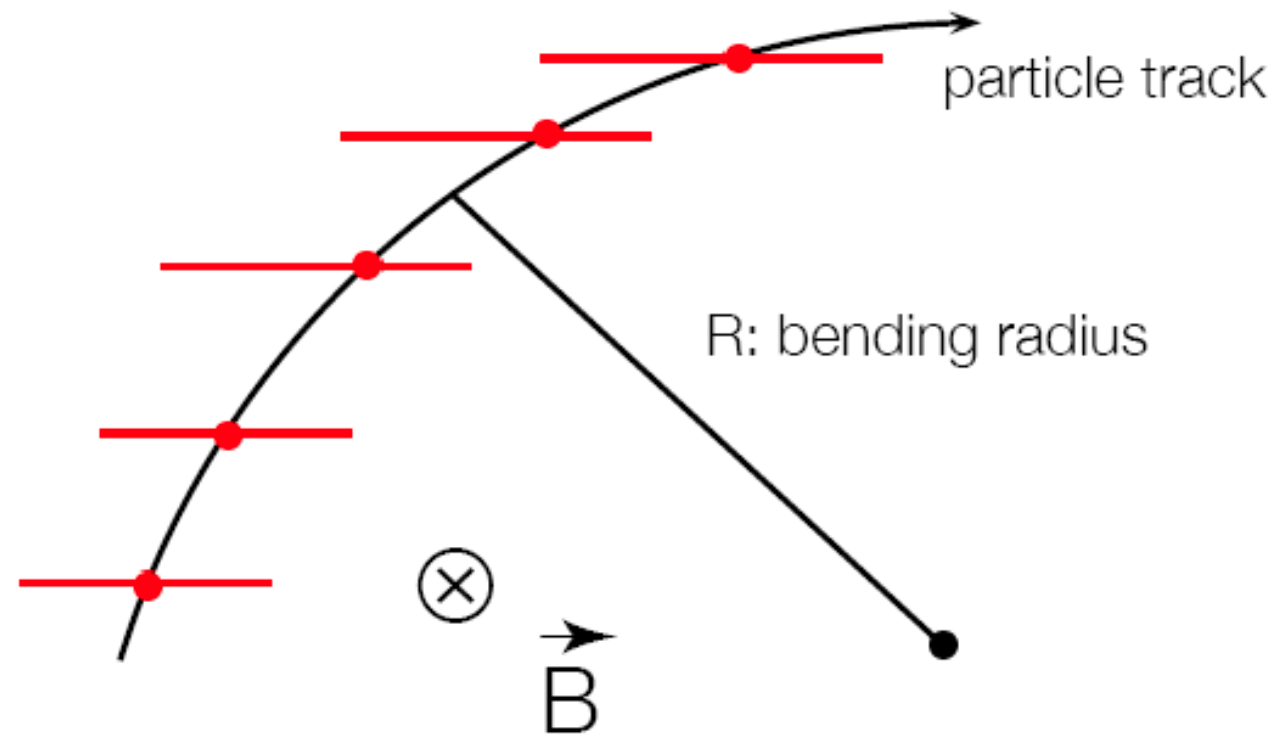
\includegraphics[width=0.75\textwidth]{\figpath/Chapter3/RadiusOfCurvature}
    \caption{Schematic view of a particle track with hits labeled.}
    \label{fig:radius_of_curvature}
\end{figure}

In each subsequent iteration the track seeding criteria is loosened and the same procedure occurs.
The looser seeding requirements boosts the tracking efficiency, while the removal of the hits from the previous iteration keeps the fake rate low due to the reduced combinatorics.
The specific seeding criteria for each iteration can also be found in table~\ref{tab:track_seeding}.
After three iterations, 90\% of charged hadron tracks within jets are reconstructed and 99.5\% of muons in the tracker acceptance are found.
Subsequent iterations loosen the constraints on the origin vertex, which allows for the reconstructions of tracks associated with a secondary vertex (i.e. $\gamma\rightarrow$\Pep\Pem~conversions, long-lived particles, nuclear interactions in the tracker material).
Tracks meeting this set of criteria can be reconstructed with as little as three hits, a \pt as low as 150\mev, and a vertex  more than 50\unit{cm} away from the beam axis.
Nevertheless, the fake rate is still kept on the order of 1\%~\cite{CMS-PAS-PFT-09-001}.

\begin{table}[htbp]
    \caption{The seed criteria used in each iteration during the 2012 run. The seed types, pair and triplet, indicate if two or three RecHits are used, respectively. The $\sigma$ in the $z_0$ criteria indicated the length of the beam spot in the $z$-direction as determined by a Gaussian fit~\cite{Tracking2012}.}
    \centering
    \begin{tabular}{llllll}
        \hline
        step  & seed type & seed sub-detectors & \pt $[\GeVcns]$ & $d_0$ [cm] & $|z_0|$ \\
        \hline
        0     & triplet   & pixel             & ${>}0.6$     & ${<}0.02$  & ${<}4.0\sigma$ \\
        1     & triplet   & pixel             & ${>}0.2$     & ${<}0.02$  & ${<}4.0\sigma$ \\
        2     & pair      & pixel             & ${>}0.6$     & ${<}0.015$ & ${<}0.09\cm$ \\
        3     & triplet   & pixel             & ${>}0.3$     & ${<}1.5$   & ${<}2.5\sigma$ \\
        4     & triplet   & pixel/TIB/TID/TEC & ${>}0.5$--0.6 & ${<}1.5$   & ${<}10.0\cm$ \\
        5     & pair      & TIB/TID/TEC       & ${>}0.6$     & ${<}2.0$   & ${<}10.0\cm$ \\
        6     & pair      & TOB/TEC           & ${>}0.6$     & ${<}2.0$   & ${<}30.0\cm$ \\
        \hline
    \end{tabular}
    \label{tab:track_seeding}
\end{table}

The tracks found will have a helical shape of with a given radius of curvature as in fig.~\ref{fig:radius_of_curvature}.
The softest, low \pt particle trajectories can form small rings, while the higher \pt particles will be bent less.
The momentum of each track can be extracted from the radius of curvature (R), given by a circular fit to the track, the magnetic field strength, as well as $\eta$ and $\varphi$ of the track at the interaction point\footnote{The $\eta$ of the track is determined as if the interaction point was at the center of the detector.}.
The following system of equations can be used to determine the particles 3-momenta at the interaction point:
\begin{equation}
    \begin{aligned}
        p_{x}&=p_{T}\cos\varphi\\
        p_{y}&=p_{T}\sin\varphi\\
        p_{z}&=p_{T}\sinh\eta\\
        p_{T}&=0.3\cdot{B}\cdot{R}
    \end{aligned}
\end{equation}

After the collection of high purity tracks is created, CMS uses these to reconstruct the location of the vertices where proton-proton interactions occurred~\cite{TRK-11-001}.
The vertex finding algorithm is agnostic to whether or not the vertices come from the main hard scatter vertex of interest or any of the pileup vertices from additional proton-proton interactions.
However, there is a need to select prompt tracks occurring near the interaction point instead of tracks from secondary vertices.
CMS requires that the significance of the transverse impact parameter $d_{0}<5$, the number of pixel hits be $\geq2$, the number of pixel and strip hits be $\geq5$, and the track $\chi^{2}<20$.
Once there is a collection of prompt tracks they are clustered together in $z$ at their closest approach to the beam spot.
A balance must be struck between vertex finding efficiency and the splitting of good vertices.
To do this, a deterministic annealing (DA) algorithm is used, which is used in cases where one wants to find the approximate global minimum of a problem with many degrees of freedom; specifically where an approximate global minimum is preferred over a more accurate local minimum.
More information about DA can be found in~\cite{Rose1998}, but simply put the process is similar to what happens when one heats a system and then slowly cools it to minimize the ``free energy,'' which in this analogy is the $\chi^{2}$ of the vertices.
In this case there is a system of $z^{T}_{i}$ with uncertainty $\sigma^{z}_{i}$ and an unknown number of vertices $z^{V}_{k}$.
There is a probability $0\leq{p_{ik}}\leq1$ for any track $i$ to be assigned to vertex $k$ and in the beginning, the algorithm assumes that every possible assignment is equally likely.
The free energy to be minimized can be found in equation~\ref{eq:DA_free_energy}, where $p_{i}$ is a constant weight for each tracks representing their consistency with originating from the beam spot and $z_{k}^{V}$ are the vertices with weights $\rho_{k}$.
\begin{equation}
    \label{eq:DA_free_energy}
    F=-T\sum_{i}^{\#tracks}p_{i}\log\sum_{k}^{\#vertices}\rho_{k}\exp\left[-\frac{1}{T}\frac{\left(z_{i}^{T}-z_{k}^{V}\right)^{2}}{{\sigma_{i}^{z}}^{2}}\right]
\end{equation}

The number of vertices can be arbitrarily large, but any extra vertices used in the method will overlap with the effective vertices already found at distinct positions.
The probability that a given track corresponds to a specific vertex is given by equation ~\ref{eq:DA_assignment_probability}.
\begin{equation}
    \label{eq:DA_assignment_probability}
    p_{ik}=\frac{\rho_{k}\exp\left[-\frac{1}{T}\frac{\left(z_{i}^{T}-z_{k}^{V}\right)^{2}}{{\sigma_{i}^{z}}^{2}}\right]}{\sum_{k'}\rho_{k'}\exp\left[-\frac{1}{T}\frac{\left(z_{i}^{T}-z_{k'}^{V}\right)^{2}}{{\sigma_{i}^{z}}^{2}}\right]}
\end{equation} 
At high temperature all tracks belong to a single vertex and all $p_{ik}$ are equal.
As $T\rightarrow0$ the each track become compatible with exactly one vertex.
The number of vertices grows each time the temperature falls below the critical temperature of a given vertex, $T_{c}^{k}$, given by equation~\ref{eq:DA_critical_temperature}, where that vertex is replaced by two nearby vertices.
As this happens the tracks are reassigned according to their probabilities before the temperature is lowered again.
The starting temperature of the whole process is chosen to be above the first critical temperature where $\rho_{1}=p_{i1}=1$.
The temperature is lowered by a cooling factor of 0.6 down to $T_{min}=4$, which balances the need to resolve all true vertices with the risk of splitting a true vertex.
\begin{equation}
    \label{eq:DA_critical_temperature}
    T_{c}^{k}=2\sum_{i}\frac{p_{i}p_{ik}}{{\sigma_{i}^{z}}^{2}}\left(\frac{z_{i}^{T}-z_{k}^{V}}{\sigma_{i}^{z}}\right)/\sum_{i}\frac{p_{i}p_{ik}}{{\sigma_{i}^{z}}^{2}}
\end{equation}
By the time the $T_{min}$ condition is reached it is still possible for a track to be assigned to multiple vertices.
Thus, for the final track assignment, the temperature is cooled to $T=1$, without more splitting of the vertices.
For a track to be assigned to a given vertex it must have a minimum probability of $0.5$ and have passed the outlier mitigation criteria.

After all of the candidate vertices are found using the DA method, the candidates with at least two tracks assigned to them are passed through the adaptive vertex fitter (AVF) to compute all of the vertex parameters.
Key among those parameters are the spacial coordinates and the number of degrees of freedom given by equation~\ref{eq:AVF_ndof}, where $w_{i}$ is a weight, between 0 and 1, given to each track depending on the likelihood that the track actually belongs to that vertex.
Additional quality requirements for a good track are $n_{dof}>4$ (at least four associated tracks), $|z|<24\unit{mm}$, and $|\rho|<2\unit{mm}$, where $\rho$ is the transverse position of the vertex~\cite{CMS-PAS-TRK-10-005}. If the track $\chi^{2}/N_{dof}<20$, then the track is matched to that vertex and only that vertex~\cite{Khachatryan:2198719}.
\begin{equation}
    \label{eq:AVF_ndof}
    n_{dof}=-3+2\sum_{i=1}^{\#tracks}w_{i}%\text{ }\forall\text{ }w_{i}\in[0,1]
\end{equation}
As mentioned before, a single vertex is classified as the ``primary'' vertex, with all other proton-proton collisions being classified as secondary, pileup vertices. The leading vertex is the one with the greatest sum of the squares of the associated tracks' transverse momenta ($\sum|\ptsup{track}|^{2}$).

The methodology above is a simplification of the actual track and vertex finding algorithms, but is sufficiently detailed for the purposes of this document. The subsequent sections will discuss how the rec hits, tracks, and vertices are used to reconstruct particles.

\section{Particle Flow}
\label{sec:particle_flow}

The CMS experiment has decided to use a holistic approach to reconstructing the event produced by a proton-proton collision.
The particle flow (PF) event reconstruction algorithm uses information from all of the sub-detectors in order to identify as accurately as possible each individual particle in the event as described in the first part of this chapter~\cite{CMS-PAS-PFT-09-001,CMS-PAS-PFT-10-001} and to reconstruct their direction and energy.
Other quantities that can be determined from a particle level reconstruction algorithm are the charged lepton isolation and the likelihood that a jet was initiated by a B hadron.
The CMS detector is ideally suited for a particle flow approach because of its extremely granular sub-detectors and high magnetic field.
This approach has been validated in~\cite{CMS-PAS-PFT-10-002,CMS-PAS-PFT-10-003,Beaudette:2014cea,CMS-PRF-14-001}, where an improvement over simpler techniques was shown each time.
The output of the PF algorithm is a list of particles known as ``PF candidates,'' which are used to build the higher level objects that physicists analyze, such as jets, taus, and \ETmiss.
Because the CMS detector is so granular, the occupancy and event complexity play almost no role in the PF algorithm efficiency.
With the current algorithm, charged-particle tracks out to \absetalt{2.6} can be reconstructed even with a \pt as low as 150\mev, all while maintaining a high reconstruction efficiency and low fake rate.
The algorithm can even identify the difference between photons and charged-particles in high multiplicity environments like jets.
This is largely due to the tracking information, which more accurately determines the \pt than the calorimeter system for for charged particles up to several hundred \gev.
Additionally, the tracker can measure the direction of a charged particle before its trajectory can be changed in the magnetic field.
Fig.~\ref{fig:particle_flow} shows, in graphical terms, how the reconstruction algorithm can classify a particle based on the sub-detectors with which it interacts.

The inputs to the PF algorithm come from the local reconstruction products, RecHits, as described at the start of chapter~\ref{ch:event_reconstruction}.
More specifically the RecHits are turned into either tracks or energy clusters, which are then used by the algorithm.
The tracks may come from the tracker, as described in section~\ref{sec:tracks_and_vertices}, or from the muon system.
The clusters are created by the calorimeter RecHits and are treated slightly different than the CaloTowers previously discussed.
A local energy maxima above a threshold value, also known as a ``cluster seed,'' is chosen as the beginning of a calorimeter cluster.
From there ``topological clusters'' are grown by adding neighboring hits above a two standard deviation threshold energy set by the subsystem to remove photo-detector noise in the ECAL (i.e. 80\mev in the barrel and up to 300\mev in the endcaps) or HCAL (i.e. 800\mev).
Some clusters are removed if its characteristics match those of an expected noise source, but otherwise a topological cluster will will create as many ``particle-flow clusters'' as there are seeds.
Energy is shared among the cells in the cluster according to the cell-cluster distance.

Once all of the tracks and clusters have been found, the two collections are associated using a ``linking algorithm'' to create ``blocks.''
First, the track is extrapolated from its last hit in the tracker subsystem to the two layers of the PS, the ECAL at a depth corresponding to the expected maximum of a typical electron shower, and to the HCAL at a depth of one interaction length.
A link is made if this extrapolated position is within the cluster boundaries, which can be enlarged by one cell size in each direction to account for non-instrumented areas, multiple scattering of low-momentum charged particles, and the uncertainty in the position of the shower maximum.
This linking algorithm is based on minimizing the $\eta-\varphi$ distance ($\Delta{R}=\sqrt{\Delta\eta-\Delta\varphi}$) between the track and cluster.
As an additional complication, tangents are drawn from the intersection between the track and the tracker layers to the ECAL.
If one of these tangents falls within an ECAL cluster then the cluster is marked as a potential Bremsstrahlung photon.
Linking between calorimeter systems (i.e. HCAL and ECAL or ECAL and PS) is done similarly, but the cluster position in the more granular system must be within the envelope of the less granular system.
A track and muon track are linked when an acceptable $\chi^{2}$ is returned by a global fit between two tracks.
If there are multiple track matches for a single muon track, then the match with the minimum $\chi^{2}$ is chosen to form a ``global muon.''
Fig.~\ref{fig:PF_linking} shows a graphical representation of what the linking algorithm sees and how the links between tracks and clusters are made.

\begin{figure}[!hbt]
    \centering
    \begin{subfigure}[t]{0.53\textwidth}
        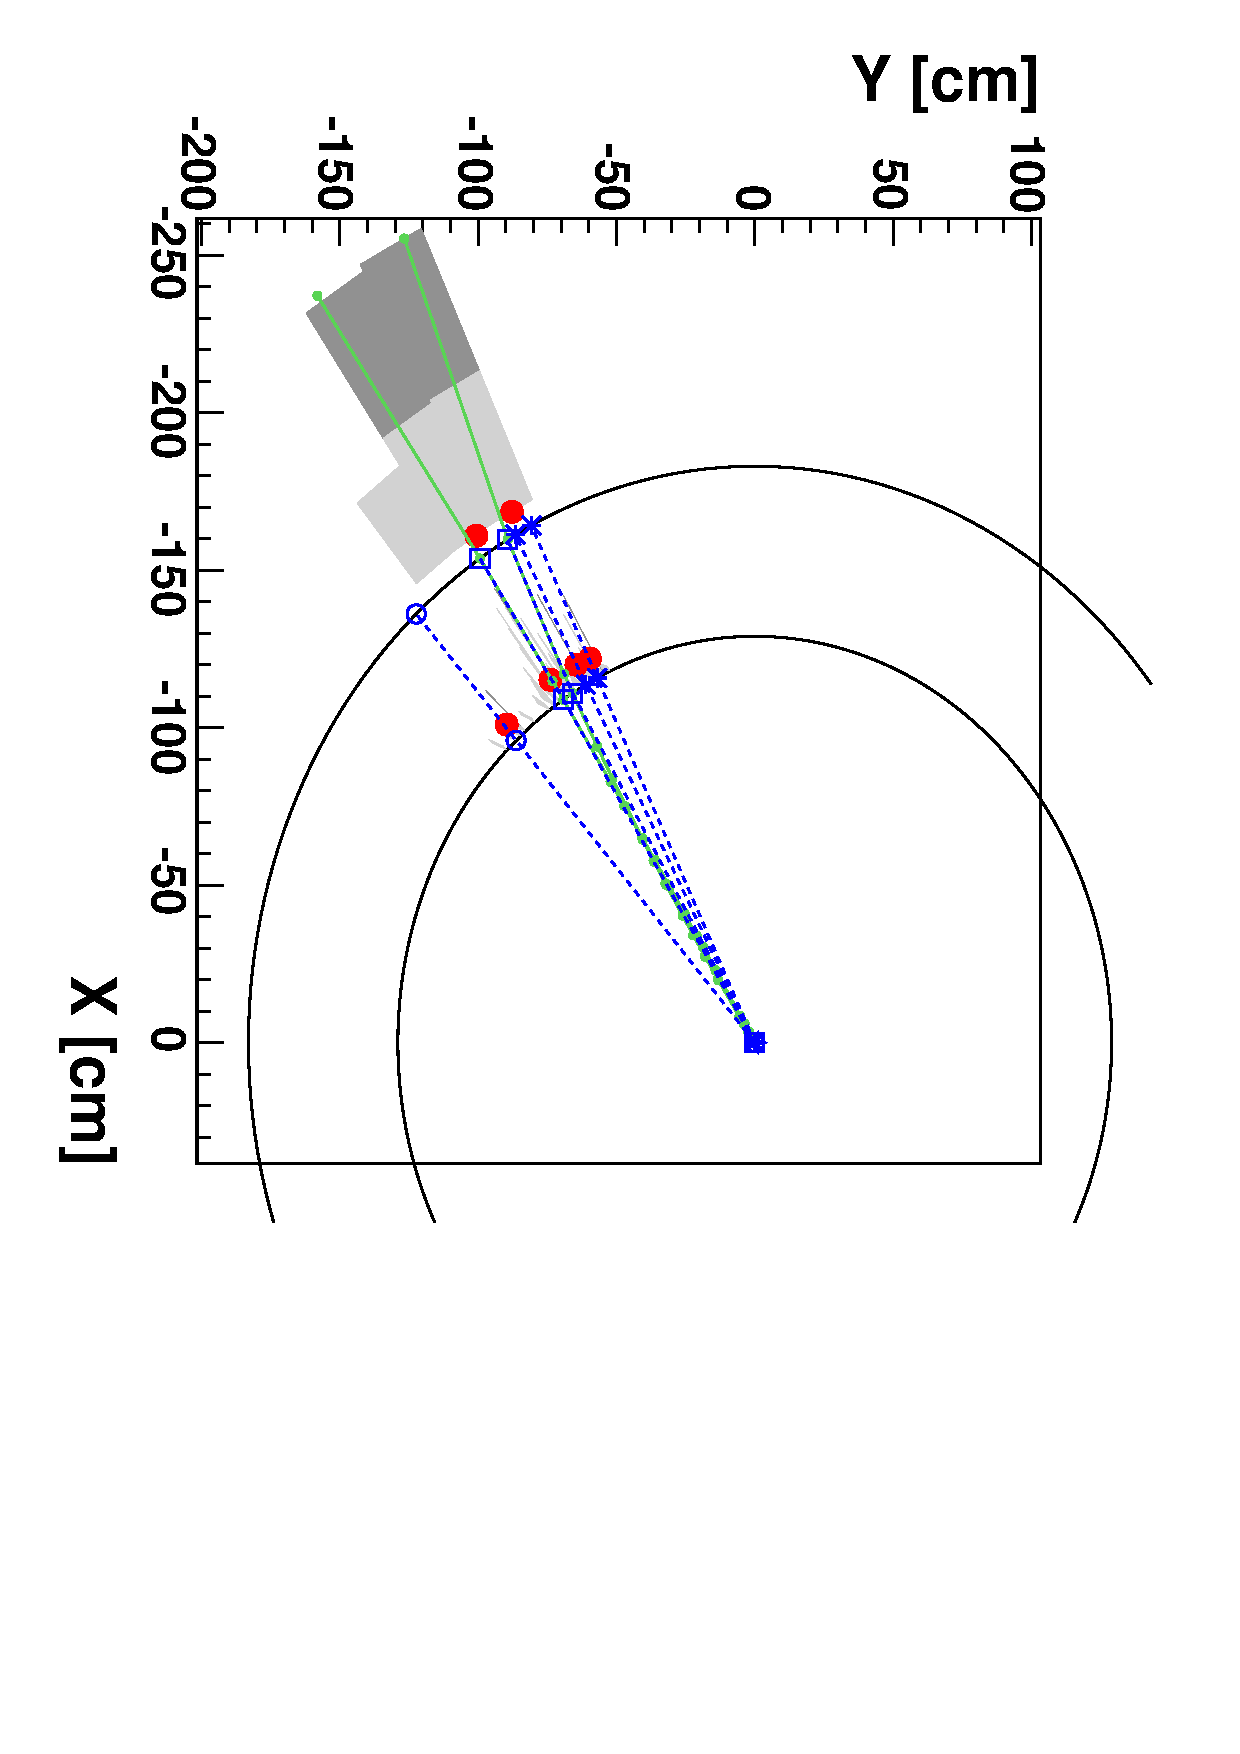
\includegraphics[width=\textwidth,angle=90]{\figpath/Chapter3/PFT-09-001_001_a.pdf}
        \caption{An $(x,y)$ view of the detector.}
        \label{fig:PF_linking_a}
    \end{subfigure}

    \begin{subfigure}[t]{0.4655\textwidth}
        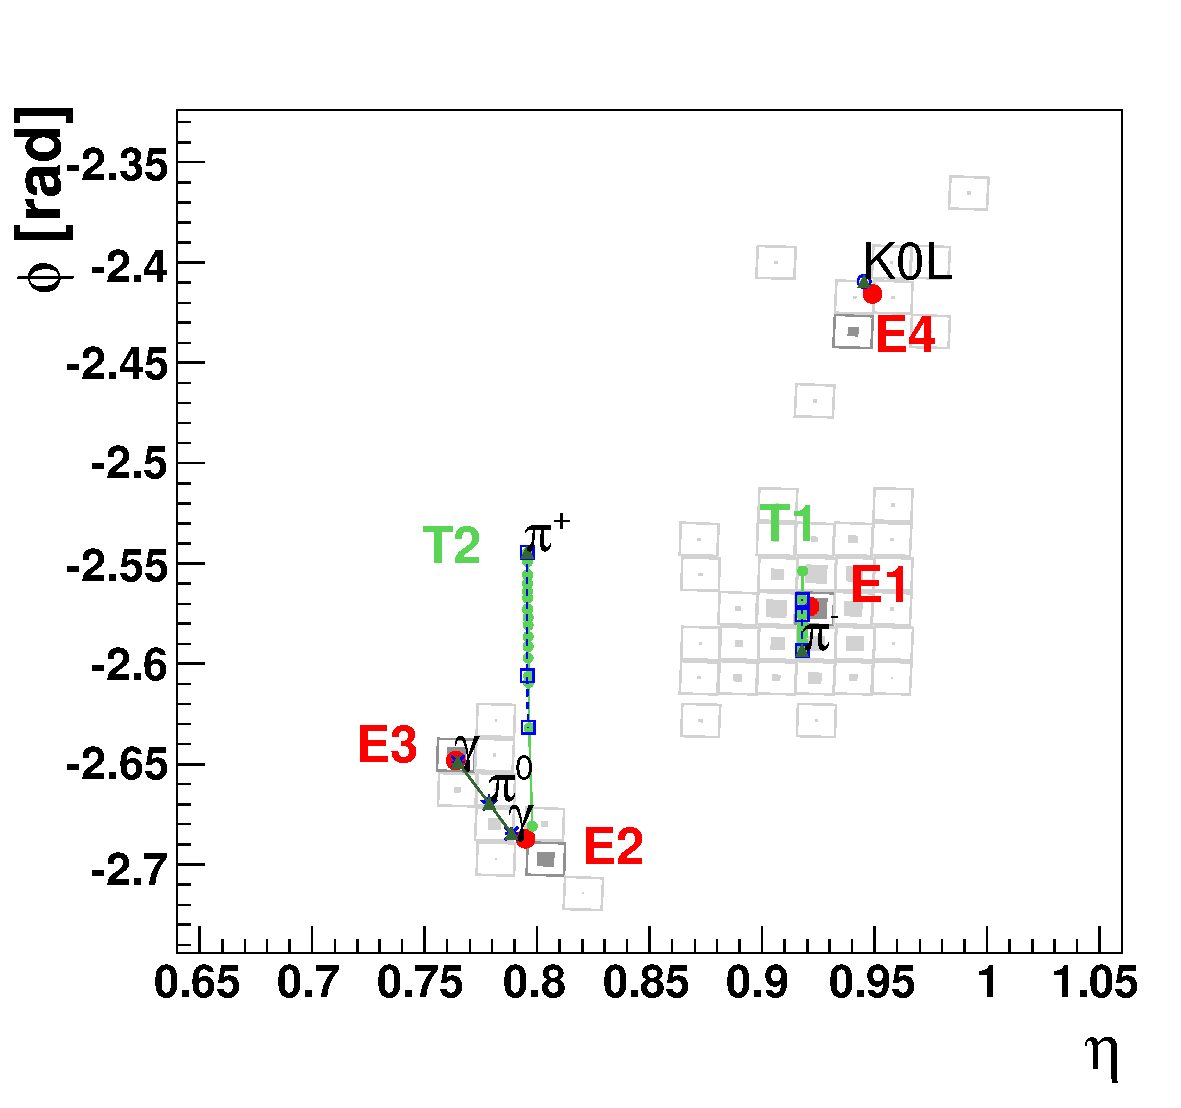
\includegraphics[width=\textwidth]{\figpath/Chapter3/PFT-09-001_001_b.pdf}
        \caption{An $(\eta,\varphi)$ view of the ECAL.}
        \label{fig:PF_linking_b}
    \end{subfigure}
    \begin{subfigure}[t]{0.4655\textwidth}
        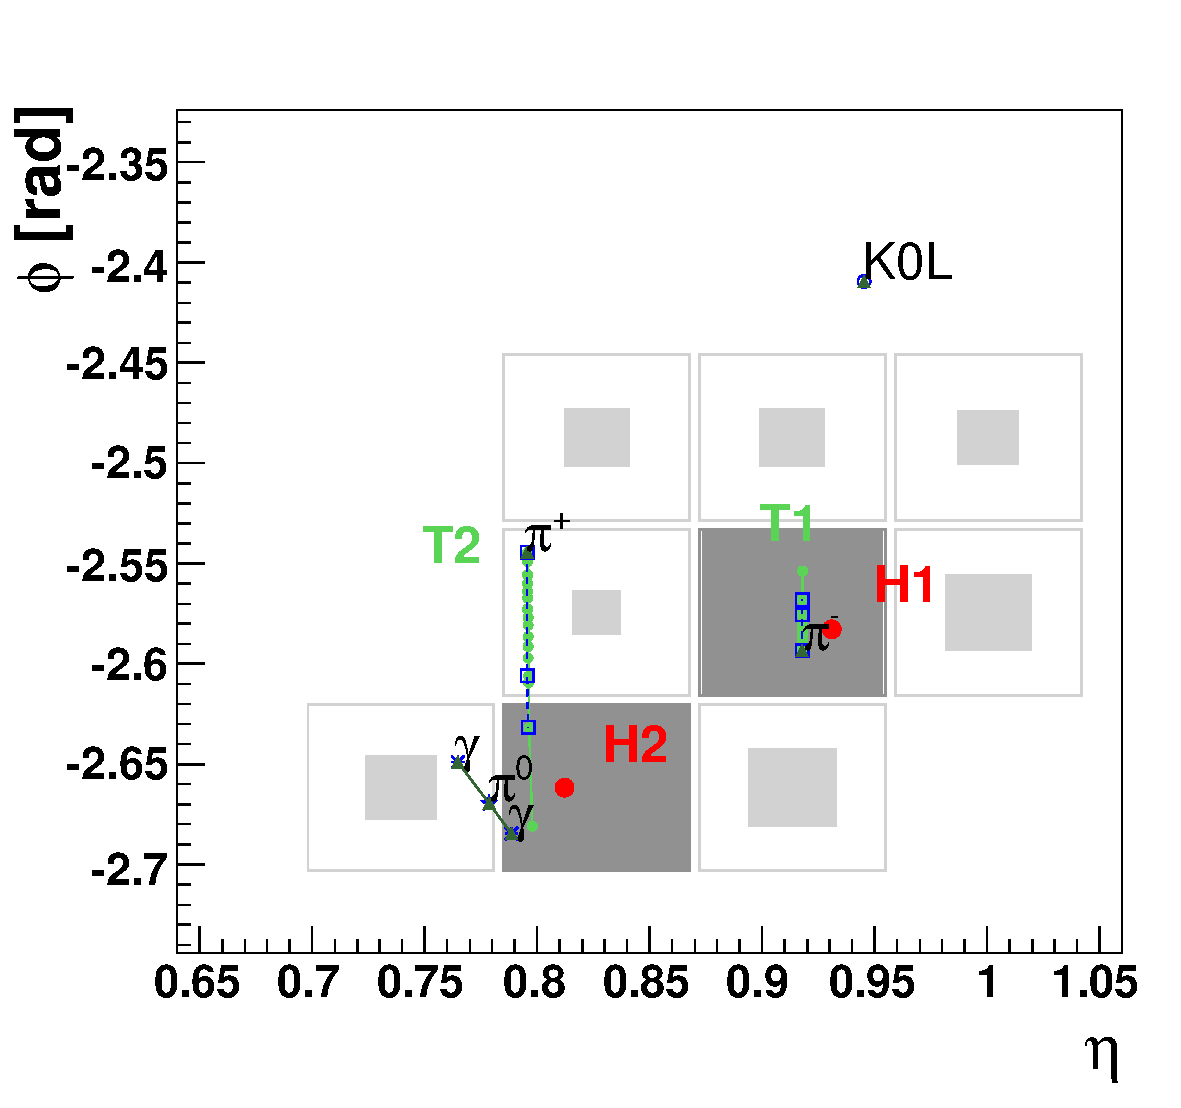
\includegraphics[width=\textwidth]{\figpath/Chapter3/PFT-09-001_001_c.pdf}
        \caption{An $(\eta,\varphi)$ view of the HCAL.}
        \label{fig:PF_linking_c}
    \end{subfigure}
    \caption{These three figures show a representation of how the PF algorithm sees a hadronic jet. (a) An $(x,y)$ view of the detector with elements from the tracker, ECAL, and HCAL shown. The ECAL and HCAL surfaces shown in (b) and (c) are represented by the concentric circles centered around the interaction point in (a). (b) shows the energy clusters from the \PKzL, \Pgpm, and the two photons from the \Pgpz decay. While the \Pgpp doesn't deposit any energy in the ECAL, it does show up as a cluster in the HCAL along with the \Pgpm (c). The tracks from these charged particles show up as vertical lines in the $(\eta,\varphi)$ plane, but as curved lines in the $(x,y)$ plane. The cluster positions are represented by dots, the simulated particles by dashed lines, and the position at which the particles impact the calorimeter surfaces by the open markers~\cite{CMS-PAS-PFT-09-001}.}
    \label{fig:PF_linking}
\end{figure}

\clearpage

The blocks are classified as a specific type of particle based on which sub-detectors were linked and then removed from the list of unclassified blocks to prevent double counting.
To begin with, if the momentum of the combined charged-particle and muon tracks is equal to the momentum of the charged-particle track alone, then the particle is classified as a PF muon.
The minimum ionization energy expected to be deposited by a muon is subtracted from the remaining clusters.
The other charged-particle tracks are checked to see if they match the properties of an electron, which is to say that electrons tend to radiate energy via bremsstrahlung, which causes the curvature of the tracks to increase as they move away from the interaction point.
A Gaussian Sum Filter (GSF) is used to match these tracks with ECAL clusters and a successful match is classified as a PF electron.
More information about the GSF and its improvements over the standard CMS tracks finding algorithms can be found at~\cite{ElectronGSF}.

Tracks which aren't matched to muons or classified as electrons are matched to clusters, if possible, and form PF charged hadrons.
In this case the total cluster energy must be similar to, but smaller than, the total track momentum.
Only the closest cluster may be linked to any given track, but a given cluster may have multiple track links due to the large granularity of the calorimeters.
The energy of charged hadrons is determined from a combination of the track momentum and the corresponding ECAL and HCAL energy, corrected for zero-suppression effects and for the response function of the calorimeters to hadronic showers.
Any excess energy remaining after removing the track energy from the clusters is assumed to come from neutral particles.
If this excess energy is in the ECAL then the neutral particle is classified as a PF photon and its energy is directly obtained from the ECAL measurement, corrected for zero-suppression effects.
After the removal of the PF photons, the remaining excesses are classified as neutral hadrons and their energy is obtained from the corresponding corrected ECAL and HCAL energy.
Clusters which are not matched to any tracks are used to make PF photons in the ECAL and neutral hadrons in the HCAL.

\section{Electrons}

Broadly speaking, the PF electron candidate identification process discussed in section~\ref{sec:particle_flow} can be considered ``tracker-driven''~\cite{CMS-PAS-EGM-10-004}.
This method is idea for low-\pt electrons and electrons in high multiplicity environments like jets.
On the other hand, high \pt electrons need an ``ECAL-driven'' approach.
In this case the ECAL clusters are grouped into ``superclusters'' for the purpose of trying to capture energy from two sources, photons produced due to bremsstrahlung and the spread of energy in $\varphi$ due to the magnetic field~\cite{ElectronReco}.
These superclusters are then matched to track seeds and a GSF is used to reconstruct the track trajectory.
The GSF is necessary to account for changes in direction due to bremsstrahlung~\cite{ElectronGSF}.
After the ECAL-driven list is created it can be compared to the list of PF electron candidates to prevent double counting.

The electron four momentum is estimated by combining the energy measurement in the ECAL, the momentum measurement in the tracker at the main interaction vertex, and the energy sum of all bremsstrahlung photons attached to the track.
The momentum resolution for electrons with $\pt \approx 45\GeV$ from $\Z \rightarrow \Pe \Pe$ decays ranges from 1.7\% for non-showering electrons in the barrel region to 4.5\% for showering electrons in the endcaps.
The dielectron mass resolution for $\Z \rightarrow \Pe \Pe$ decays when both electrons are in the ECAL barrel is 1.9\%, and is 2.9\% when both electrons are in the endcaps.~\cite{Khachatryan:2015hwa}.

Only electron selection has been discussed so far.
However, once there is a complete list of electron candidates, quality cuts are imposed to identify genuine electrons~\cite{ElectronCutBased,ElectronMVABased,ElectronConversionVeto}.
There are two similar methods for evaluating these quality requirements.
One is a purely cut based technique and the other merges these requirements, plus some additional variables, into a single MVA based training.
This analysis used the MVA based training in order to extract as much performance from the selection cuts as possible.
However, it is still informative to list the cut based requirements since they are all used inside of the MVA training.
The $\eta$ width of the supercluster, $\sigma_{i{\eta}i{\eta}}$, is taken from the covariance matrix of a weighted difference between the $\eta$ positions of the crystals and the seed cluster.
A modified $\eta$ is used in this calculation to account for the crystal spacing and each crystals contribution is weighted by $\log\left(E_{crystal}/E_{sc}\right)$~\cite{EgammaShowerShape}.
Two additional variables are calculated as the differences between the positions of the supercluster, $\left(\eta_{sc},\varphi_{sc}\right)$, and the extrapolated track, $\left(\eta_{in}^{extrap},\varphi_{in}^{extrap}\right)$, thus defined as $|\Delta\eta_{in}|=|\eta_{sc}-\eta_{in}^{extrap}|$ and $|\Delta\varphi_{in}|=|\varphi_{sc}-\varphi_{in}^{extrap}|$.
The ratio of the leakage energy, H, in the HCAL tower behind the ECAL seed cluster is compared to the energy of that seed cluster in the variable $H/E$.
The transverse and longitudinal impact parameters compared to the associated vertex, $d_{0}^{vtx}$ and $d_{z}^{vtx}$, and a comparison of the electron energy and momentum, $|1/E-1/p|$, are used.
Both identification schemes also make use of the PF based isolation variable shown in equation~\ref{eq:PFIsolation_electron}. However, rather than using the base isolation value, the relative isolation $I_{e}^{PF}/\pt^{e}$ is used.
The isolation is variable is simply the sum of the \pt of the charged hadron (CH), neutral hadron (NH), and photon ($\gamma$) PF candidates within a cone of $\Delta{R}<0.3$ around the electron candidate.
The expected amount of energy due to pileup is then removed by multiplying the median energy density by the electron effective area, $A_{eff}$, but it protected from becoming a negative value.
\begin{equation}
\label{eq:PFIsolation_electron}
I_{e}^{PF}=\sum_{\Delta{R}<0.3}\pt^{\left(CH\right)}+max\left(\sum_{\Delta{R}<0.3}\pt^{\left(NH\right)}+\sum_{\Delta{R}<0.3}\pt^{\left(\gamma\right)}-{\rho}A_{eff},0\right)
\end{equation}

A set of values for the identification requirements is called a working point (WP) and there are several WP based upon the desired identification efficiency and fake rate.
This analysis makes use of the tight working point for the selected electron and the loose working point to veto on additional electrons.
Table~\ref{tab:electron_id_cut} lists the cut based identification requirements for the tight and loose WP.
Similarly, table~\ref{tab:electron_id_mva} lists the requirements for the MVA based identification.
In addition to the identification requirements, selected electrons must have a $\pt>27\gev$ and be in the barrel, \absetaltss{1.4442}{sc}, or endcap, \absetass{1.566}{2.5}{sc}.
The must also pass a conversion veto to make sure the aren't produced by a converted photon.
Loose electrons have the same $eta$ and conversion requirements, but are only required to have a $\pt>15\gev$.
The \pt requirements are selected to match the HLT requirements of the PD listed in section~\ref{sec:data}.

\begin{table}[htbp]
    \caption{Cut based electron identification requirements for the tight and loose working points.}
    \centering
    \begin{tabular}{lllll}
        \hline
        \multirow{3}{*}{Cut Variable} & \multicolumn{4}{c}{Cut Value} \\\cline{2-5}
                                      & \multicolumn{2}{c}{Tight}     & \multicolumn{2}{c}{Loose} \\\cline{2-5}
                                      & Barrel & Endcap & Barrel & Endcap \\
        \hline
        $I_{e}^{PF}/\pt^{(e)}<$       & 0.1    & 0.1    & 0.15   & 0.15   \\
        $\sigma_{i{\eta}i{\eta}}<$    & 0.01   & 0.03   & 0.01   & 0.03   \\
        $|\Delta\varphi_{in}|<$       & 0.03   & 0.02   & 0.8    & 0.7    \\
        $|\Delta\eta_{in}|<$          & 0.004  & 0.005  & 0.007  & 0.01   \\
        $H/E<$                        & 0.12   & 0.1    & 0.15   & 0.07   \\
        $|d_{0}^{vtx}|<$              & 0.02   & 0.02   & 0.04   & 0.04   \\
        $|d_{z}^{vtx}|<$              & 0.1    & 0.1    & 0.2    & 0.2    \\
        $|1/E-1/p|<$                  & 0.05   & 0.05   & -      & -      \\
        \hline
    \end{tabular}
    \label{tab:electron_id_cut}
\end{table}

\begin{table}[htbp]
    \caption{MVA based electron identification requirements for the tight and loose working points. The tight MVA requirements were trained using triggering electrons whereas the loose MVA requirements, usually used as a veto, were trained on non-triggering electrons.}
    \centering
    \begin{tabular}{lllll}
        \hline
        \multirow{3}{*}{Supercluster Pseudorapidity} & \multicolumn{4}{c}{Cut Value} \\\cline{2-5}
                                        & \multicolumn{2}{c}{Tight}         & \multicolumn{2}{c}{Loose} \\\cline{2-5}
                                        & MVA      & $I_{e}^{PF}/\pt^{(e)}$ & MVA      & $I_{e}^{PF}/\pt^{(e)}$ \\
        \hline
        $\absetaltss{0.8}{sc}$          & $>$0.977 & $<$0.093               & $>$0.877 & $<$0.426 \\
        $\absetass{0.8}{1.479}{sc}$     & $>$0.956 & $<$0.095               & $>$0.811 & $<$0.481 \\
        $\absetass{1.479}{2.5}{sc}$     & $>$0.966 & $<$0.171               & $>$0.707 & $<$0.390 \\
        \hline
    \end{tabular}
    \label{tab:electron_id_mva}
\end{table}

\section{Muons}

In addition to using the PF algorithm to identify muon candidates, CMS uses two supplementary methods to identify high and low-momentum muon candidates~\cite{CMS-PAS-MUO-10-002}. The union of these collections will me used for the final muon reconstruction. To capture the low-momentum muons, charged particle tracks which have a \pt and $p$ above a threshold are extrapolated out to the muon sub-detector. If the track position matched a track segment in the muon sub-detector, then the track is made into ``tracker muon.'' The other method, able to capture the high-momentum muons, is to find a match in the tracker for the standalone muons made by the muon sub-detector, which is the reverse of the previous method. If a match is found, then the candidate is considered a ``global muon'' and a global fit of the two tracks is made to improve the momentum measurement and resolution. The global muons, tracker muons, and standalone muons are then combined into a single collection which avoids double counting.

Just like for the electrons, there are identification requirements which each muon must pass. This helps to remove cosmic ray muons, muons from heavy flavor decays, and leakage from hadronic showers which may enter the muon collection. Just like the electrons, the the distance between the primary vertex and the transverse and longitudinal impact parameters, $d_{0}^{vtx}$ and $d_{z}^{vtx}$, are used. Additionally, there are requirements on the number of hits in the muon system, the number of stations used in the muon system, the number of pixel hits in the tracker, the overall number of tracker hits, and the reduced $\chi^{2}$ of the global muon fit. The isolation, which can be seen in equation~\ref{eq:PFIsolation_muon}, is calculated using the PF candidates within a cone of $\Delta{R}<0.4$ around the muon.
\begin{equation}
\label{eq:PFIsolation_muon}
I_{\mu}^{PF}=\sum_{\Delta{R}<0.4}\pt^{\left(CH\right)}+max\left(\sum_{\Delta{R}<0.4}\pt^{\left(NH\right)}+\sum_{\Delta{R}<0.4}\pt^{\left(\gamma\right)}-{\Delta\beta\sum_{\Delta{R}<0.4}}\pt^{\left(PU\right)},0\right)
\end{equation}
The variable is very similar to the one used for electrons except that instead of an effective area pileup correction, the muons use a pileup correction based on the sum \pt of the charge particles which don't come from the same vertex as the muon candidate. The $\Delta\beta$ term is set to 0.5 and is the ratio of charged to neutral particles in pileup~\cite{CMS-PAS-PFT-10-002}.

The identification requirements for electrons also rely on two WP, a set of tight cuts to select for muons to use in the analysis and a set of loose cuts to veto on additional muons. One again, additional \pt and $\eta$ requirements are imposed on the tight and loose muons to ensure that they match the requirements of the PD as stated in~\ref{sec:data}. The tight muons must have $\pt>24\gev$ and be within \absetalt{2.1} whereas the loose muons must have $\pt>10\gev$ and be within \absetalt{2.5}. The cuts used to identify good, prompt muons are listed in table~\ref{tab:muon_id_cut}.

\begin{table}[htbp]
    \caption{Cut based muon identification requirements for the tight and loose working points.}
    \centering
    \begin{tabular}{lll}
        \hline
        \multirow{2}{*}{Cut Variable}               & \multicolumn{2}{c}{Cut Value} \\\cline{2-3}
                                                    & \multicolumn{1}{c}{Tight}     & \multicolumn{1}{c}{Loose} \\\cline{2-3}
        \hline
        Is PF muon                                  & True        & True                        \\
        Muon category                               & Global muon & Global muon OR tracker muon \\
        $I_{\mu}^{PF}/\pt^{(\mu)}<$                 & 0.12        & 0.2                         \\
        $|d_{0}^{vtx}|<$                            & 0.02        & -                           \\
        $|d_{z}^{vtx}|<$                            & 0.5         & -                           \\
        Global track fit $\chi^{2}/n_{\text{dof}}<$ & 10          & -                           \\
        Global track fit $n_\text{muon segment}>$   & 0           & -                           \\
        $n_{hits}\left(\text{pixel}\right)>$        & 0           & -                           \\
        $n_{layers}\left(\text{tracker}\right)>$    & 5           & -                           \\
        $n_{stations}\left(\text{muon}\right)>$     & 1           & -                           \\
        \hline
    \end{tabular}
    \label{tab:muon_id_cut}
\end{table}

\section{Jets}
\label{sec:jets}

The protons that make up the LHC beams are bound states of quarks and gluons, which are particles that carry color charge.
If, during a proton-proton collision, a quark or gluon is freed, it must create other colored particles to combine with and form color singlet bound states, hadrons, in a process known as hadronization.
This is because a colored state cannot exist alone due to QCD confinement, which only allows for free colorless states.
The cascade of particle production will continue until there are no free color states and there is not enough energy to continue hadronizing.
The hadronization products themselves may still decay into other particles, including colorless leptons and photons.
The CMS detector will not see the initiating parton, but it will certainly measure this cascade of particles as a narrow cluster of tracks and energy, which are collectively referred to as a jet~\cite{Salam:2009jx}.

\begin{figure}[!hbt]
    \centering
    \begin{subfigure}[t]{0.32\textwidth}
        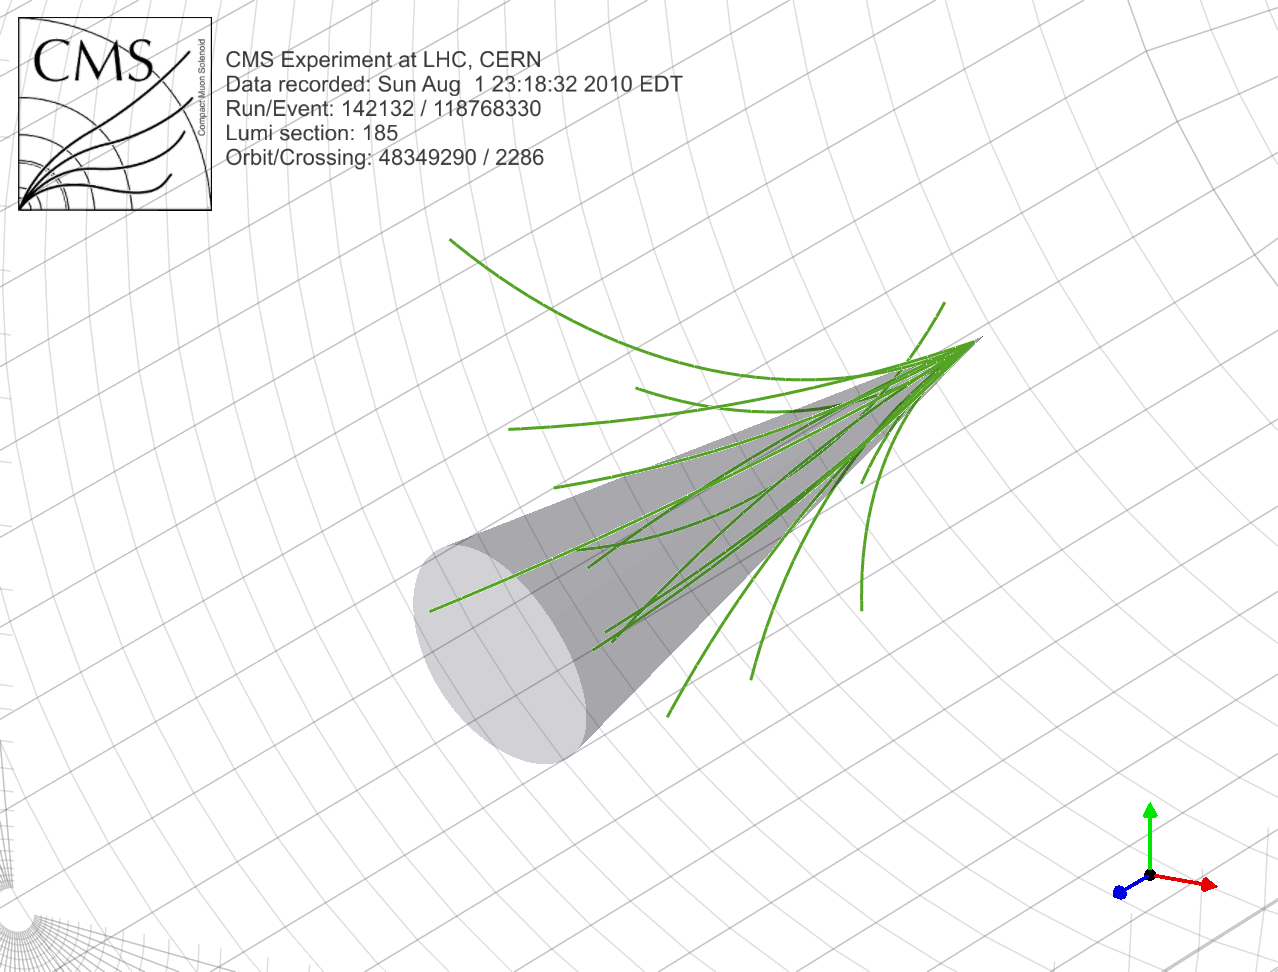
\includegraphics[width=\textwidth]{\figpath/Chapter3/JetConeWithTracks.png}
        \caption{}
        \label{fig:jc_track}
    \end{subfigure}
    \begin{subfigure}[t]{0.32\textwidth}
        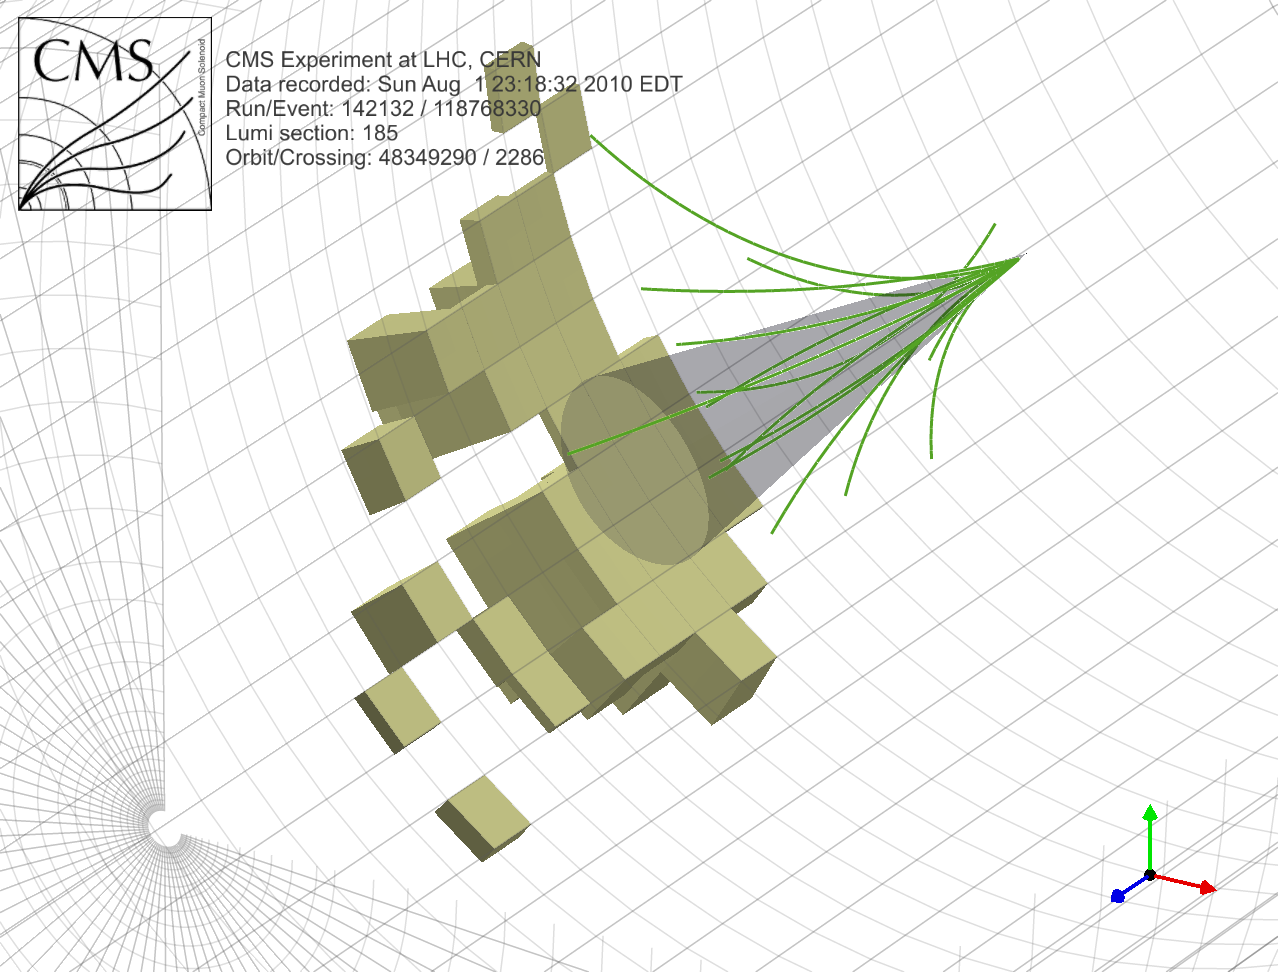
\includegraphics[width=\textwidth]{\figpath/Chapter3/JetConeWithTracksAndECAL.png}
        \caption{}
        \label{fig:jc_track_ecal}
    \end{subfigure}
    \begin{subfigure}[t]{0.32\textwidth}
        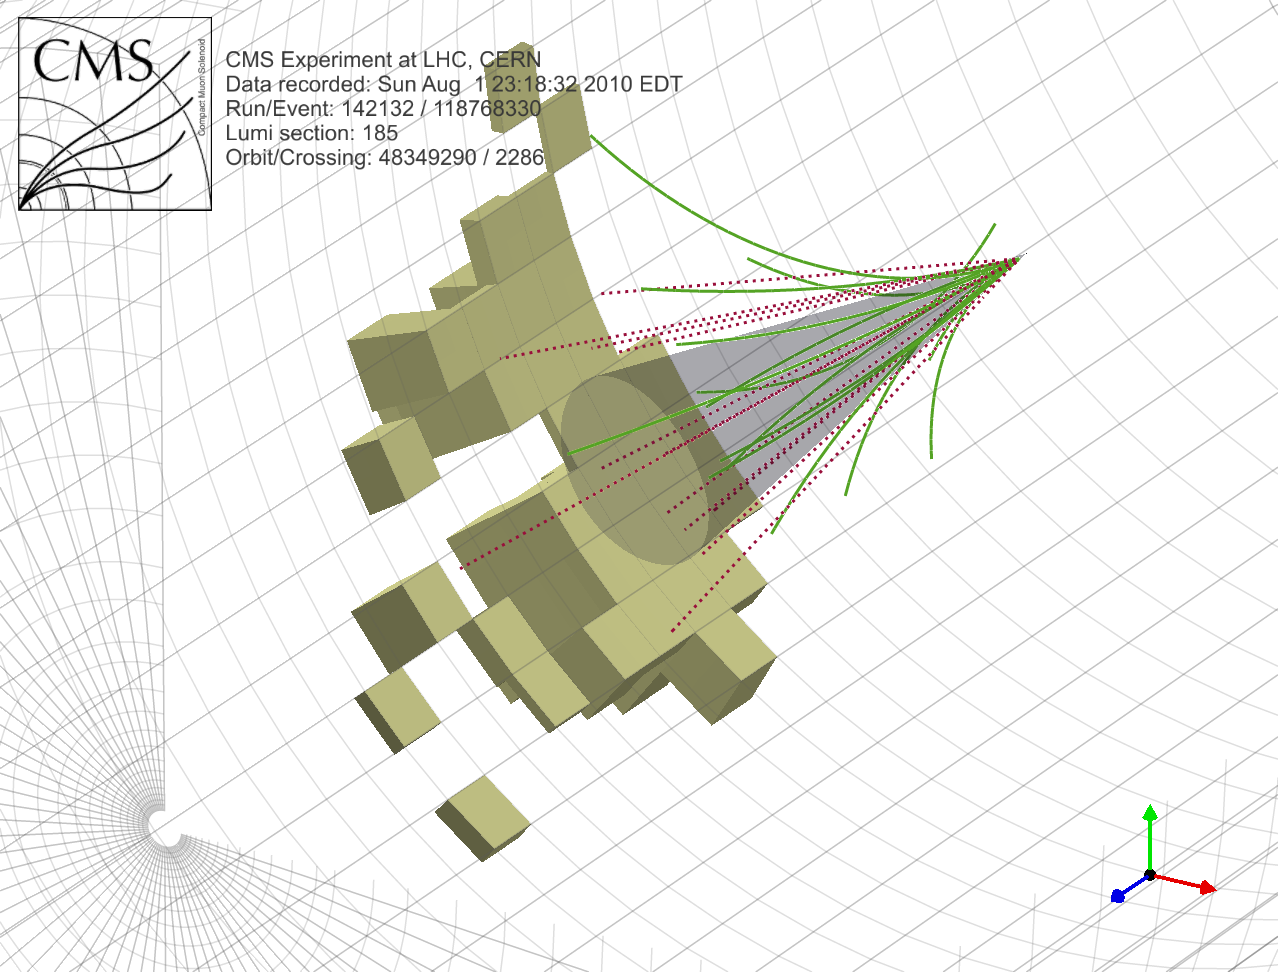
\includegraphics[width=\textwidth]{\figpath/Chapter3/JetConeWithTracksAndPhotonsAndECAL.png}
        \caption{}
        \label{fig:jc_track_photon_ecal}
    \end{subfigure}

    \begin{subfigure}[t]{0.32\textwidth}
        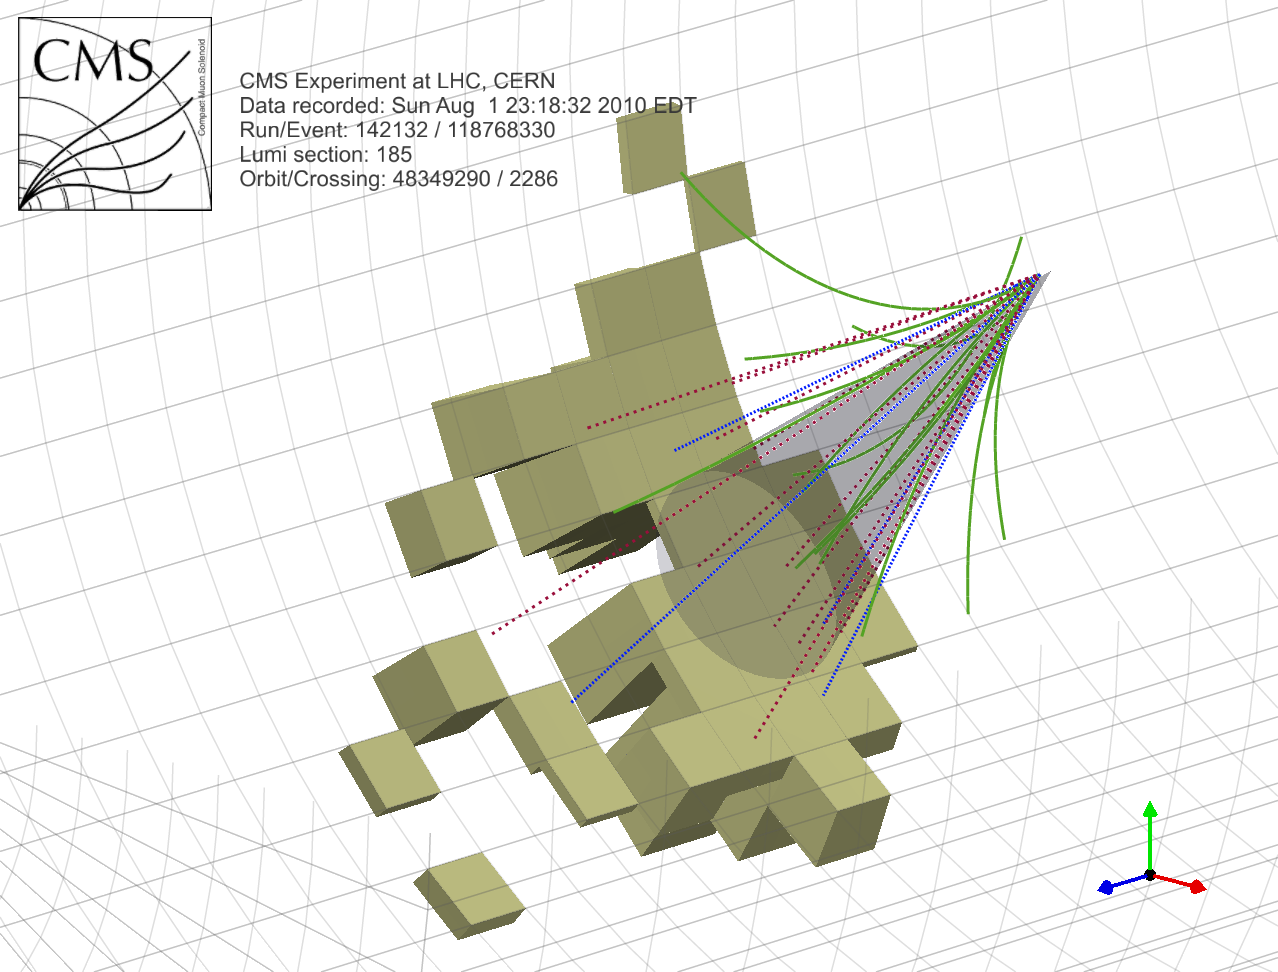
\includegraphics[width=\textwidth]{\figpath/Chapter3/JetConeWithTracksAndPhotonsAndNeutralHAndECAL.png}
        \caption{}
        \label{fig:jc_track_photon_neutralH_ecal}
    \end{subfigure}
    \begin{subfigure}[t]{0.32\textwidth}
        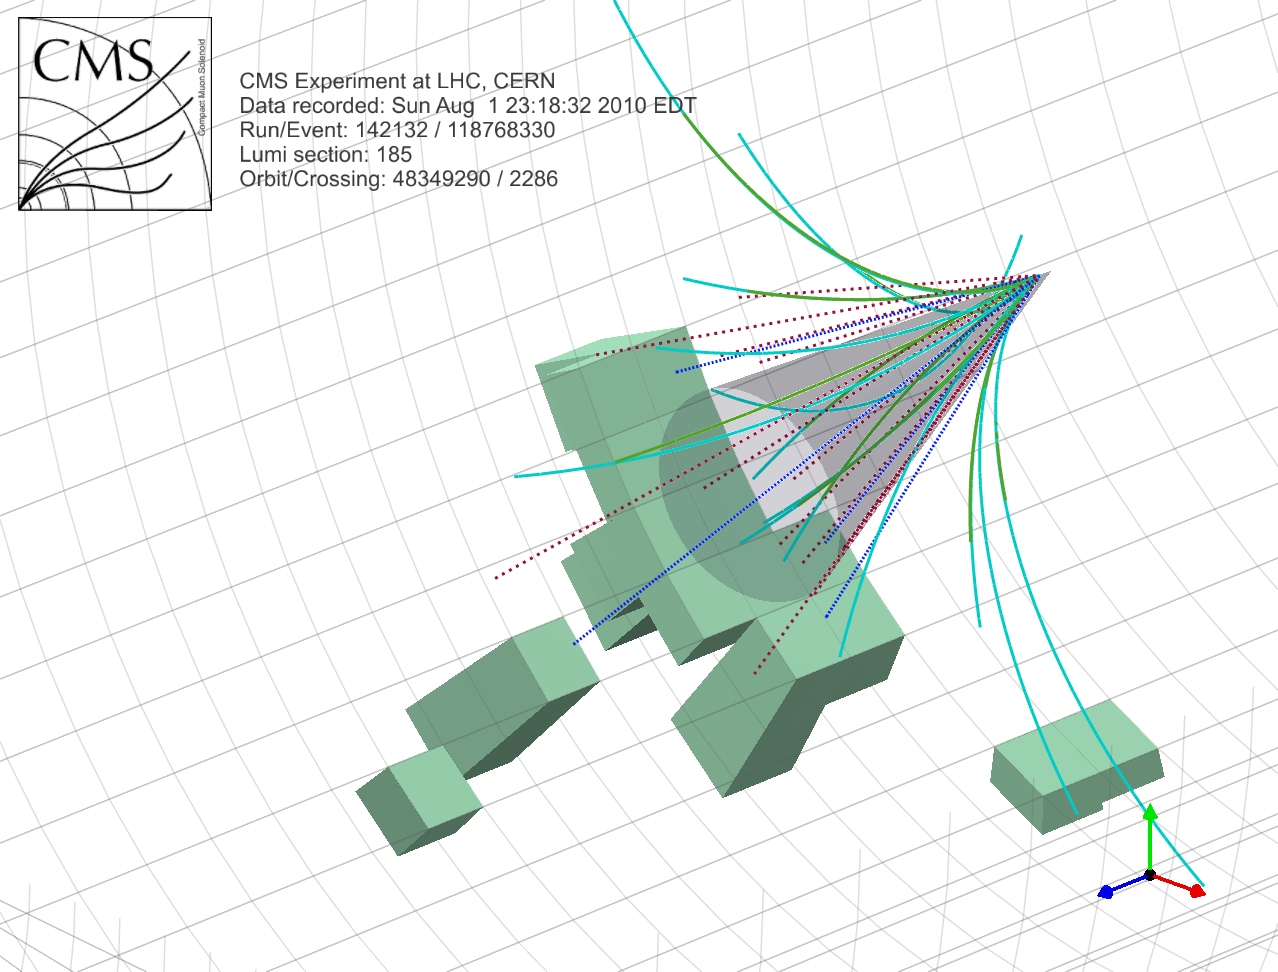
\includegraphics[width=\textwidth]{\figpath/Chapter3/JetConeWithTracksAndPhotonsAndNeutralHAndChargedHAndHCAL.png}
        \caption{}
        \label{fig:jc_track_photon_neutralH_chargedH_hcal}
    \end{subfigure}
    \begin{subfigure}[t]{0.32\textwidth}
        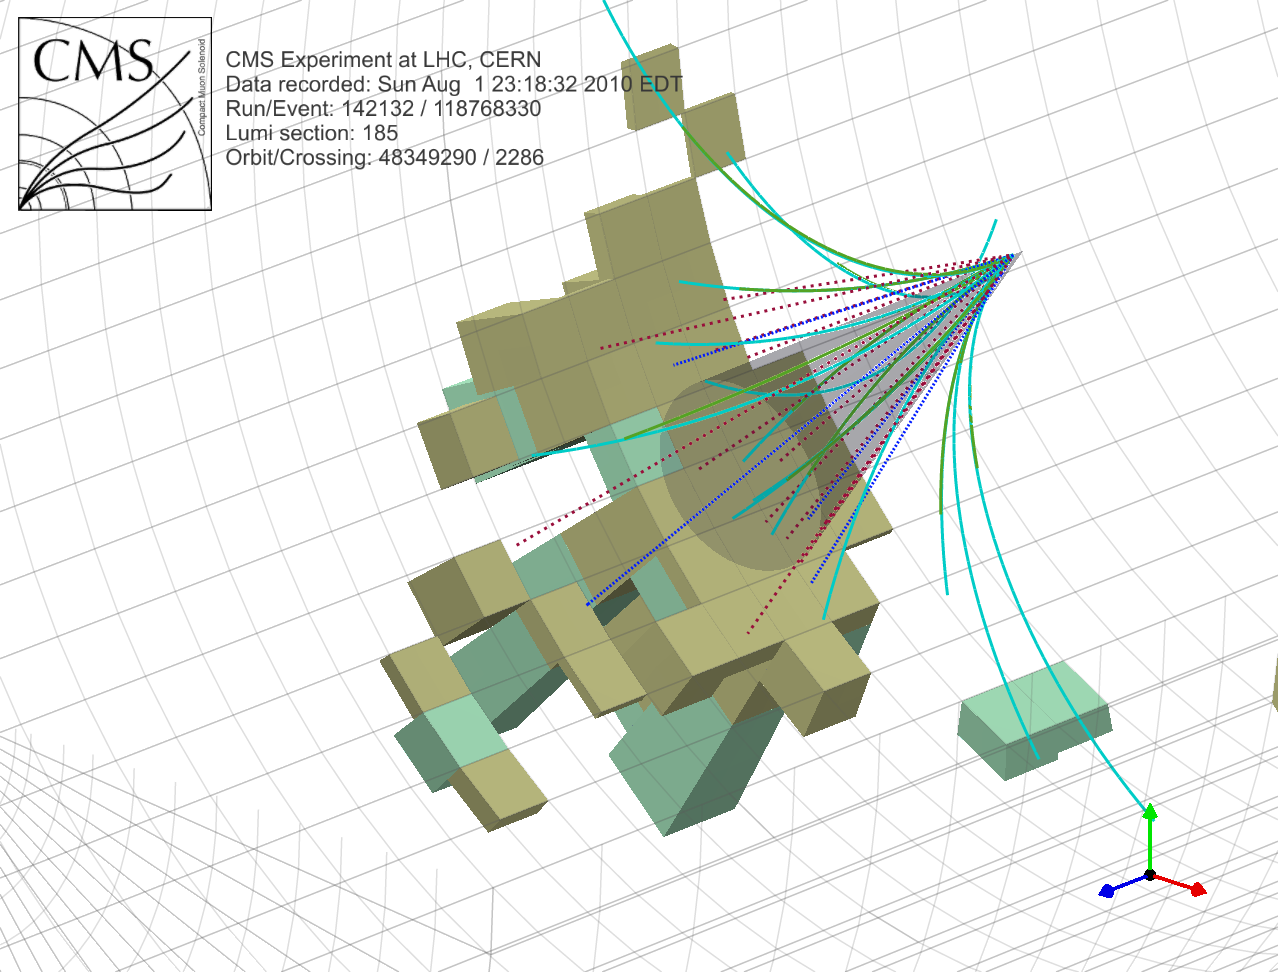
\includegraphics[width=\textwidth]{\figpath/Chapter3/JetConeAll.png}
        \caption{}
        \label{fig:jc_all}
    \end{subfigure}

    \begin{subfigure}[t]{0.32\textwidth}
        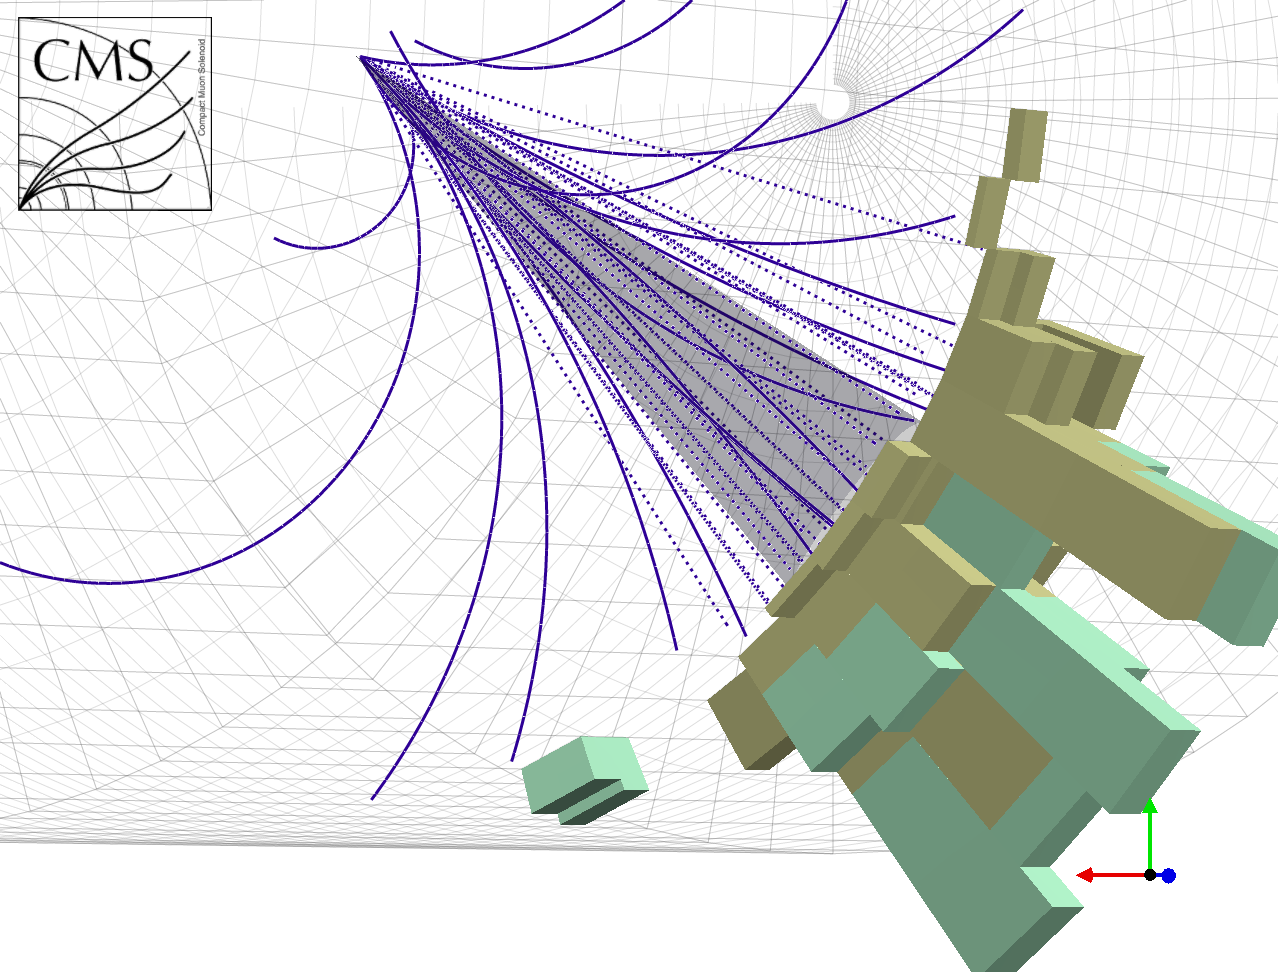
\includegraphics[width=\textwidth]{\figpath/Chapter3/JetConeAndPFJetCALVIEW1.png}
        \caption{}
        \label{fig:jc_PFjet1}
    \end{subfigure}
    \begin{subfigure}[t]{0.32\textwidth}
        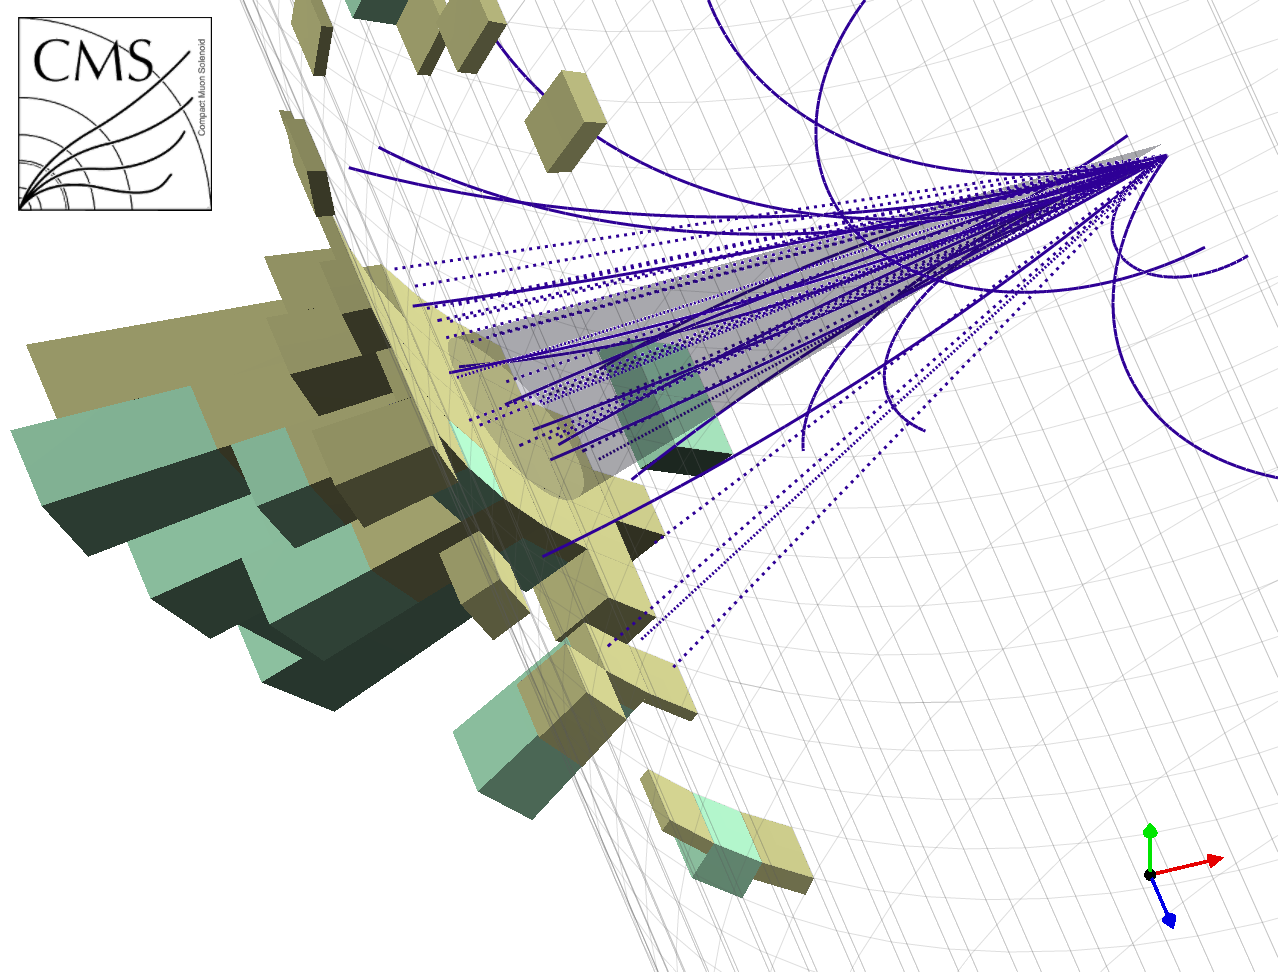
\includegraphics[width=\textwidth]{\figpath/Chapter3/JetConeAndPFJetCALVIEW3.png}
        \caption{}
        \label{fig:jc_PFJet3}
    \end{subfigure}
    \begin{subfigure}[t]{0.32\textwidth}
        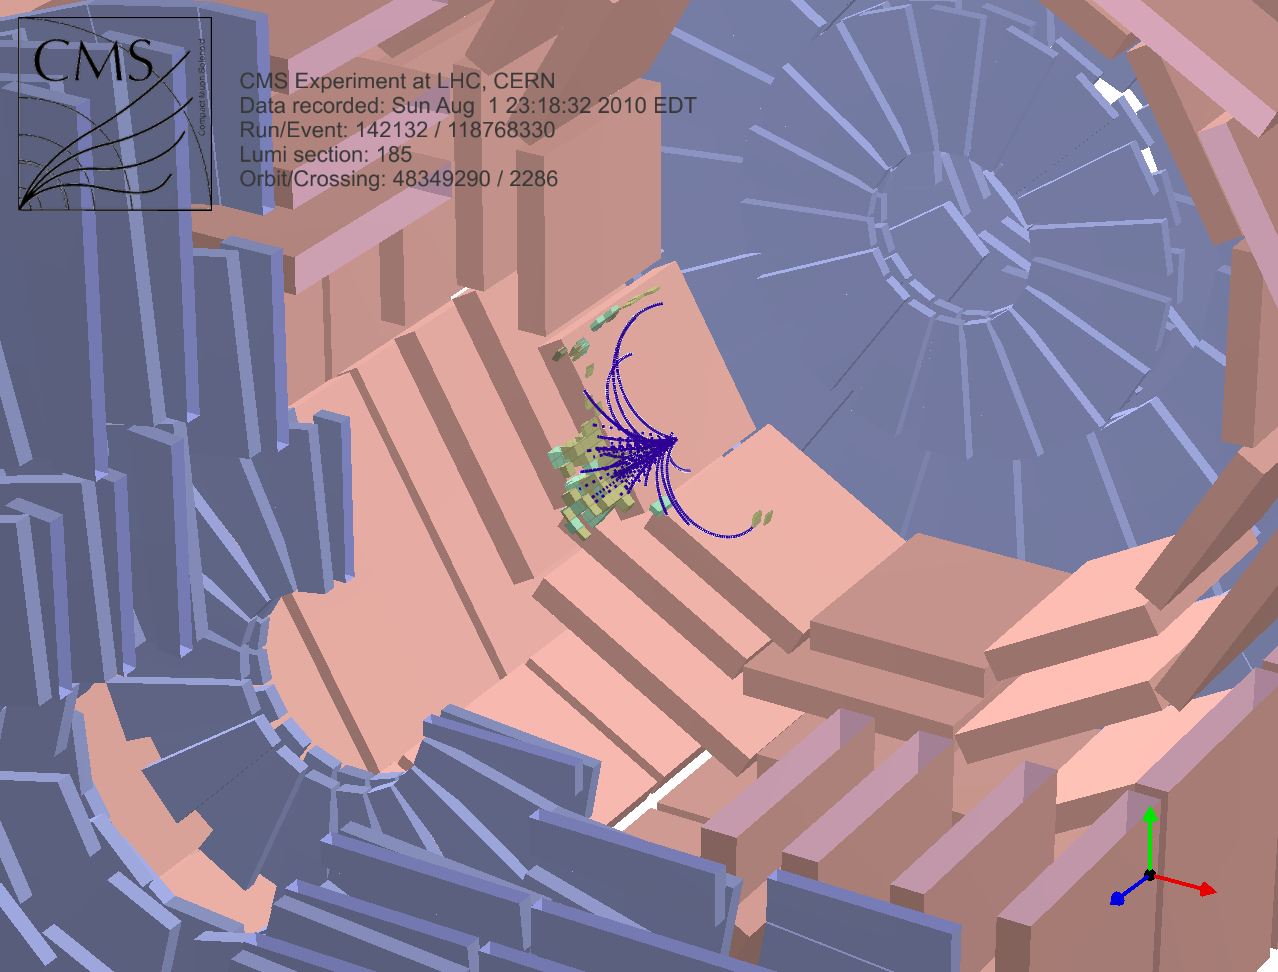
\includegraphics[width=\textwidth]{\figpath/Chapter3/JetWithFullDetector.png}
        \caption{}
        \label{fig:jet_fullDetector}
    \end{subfigure}
    \caption{Different views of the same 115\gev PF jet are shown with varying amounts of information displayed. The panels are ordered sequentially from left to right and top to bottom where each subsequent panel includes additional information. The image is of a jet with its (a) tracks, (b) ECAL deposits, (c) photon candidates, (d) neutral hadrons. Panel (e) shows the jet with its charged hadrons, but replacing the ECAL deposits for the HCAL deposits. Panels (f)-(h) show various views of the same jet with all of its constituents, while panel (i) shows the jet as it would appear in the CMS detector. The distance between the primary vertex and the interior of the red muon chambers is 7.5\unit{m} and the calorimeter deposits are scaled to about 10\unit{\gev/m}~\cite{Dorney2014}.}
    \label{fig:BuildingAPFJet}
\end{figure}

While the best way to cluster the cascade is still an open topic of discussion\footnote{Researchers are constantly asking themselves, "What is a jet?" The question is referring more to the idea of how to reconstruct a jet rather than the concept of a jet.}, this analysis clusters PF candidates using the anti-k\textsubscript{T} algorithm~\cite{Cacciari:2008gp} as defined in the \textsc{Fast}\textsc{Jet} package~\cite{Cacciari:2011ma}\footnote{In addition to providing fast, sequential clustering algorithms, the \textsc{Fast}\textsc{Jet} package is able to calculate the jet area, which is a non-trivial quantity~\cite{Cacciari2008}.}.
The anti-k\textsubscript{T} is a sequential recombination clustering algorithm which is both infrared and collinear safe.
Infrared safety means that the jet clustering algorithm is insensitive to the emission of soft, wide angle particles.
In other words, the jet is invariant under $\vec{p}_{i}\rightarrow\vec{p}_{j}+\vec{p}_{k}$, where the particle with momentum $\vec{p}_{i}$ split into two particles, each carrying momentum $\vec{p}_{j}$ and $\vec{p}_{k}$ respectively.
As an example, two jets should not be merged together just because one of them produced a 1\gev particle between them.
Collinear safety means that if there is a splitting which results in two parallel high-\pt particles, a single jet is produced and the jet properties will not be different from a jet where this splitting did not occur.
When an algorithm obeys these two properties, they are referred to as being IRC safe.
Simply put, the anti-k\textsubscript{T} algorithm results in jets which have physical properties (i.e. \pt, mass, etc.) that are representative of the partons in the event.

The use of PF candidate, with their built in tracking information, provides a huge benefit to the reconstruction and clustering of jets in CMS. About 65\% of the energy within a jet is carried by the charged particles and thus a lot of information about a jet comes from the tracker.\footnote{25\% of the energy is carried by photons and the remaining 10\% is carried by neutral hadrons.} An alternative to clustering PF candidates is to cluster the energy deposits in the calorimeter towers, but that provides both less spacial information as well as a lower response, where jet response is defined as $\left<\left(\ptsup{reco}-\ptsup{gen}\right)/\ptsup{gen}\right>$ and $\ptsup{reco}$ ($\ptsup{gen}$) is the reconstructed (generated) \pt. Fig.~\ref{fig:PFVsCaloJetResponse} shows a comparison of the PF based jet response (PF jets) versus calorimeter based jet responses (calo jets). The use of tracking information also improves the jet resolution, where typical values for a PF jet are 15\% at 10\GeV, 8\% at 100\GeV, and 4\% at 1\TeV. This is compared to about 40\%, 12\%, and 5\% when using calo jets~\cite{CMS-PAS-PFT-09-001}. A comparison of the resolution curves can be see in fig.~\ref{fig:PFVsCaloJetResolution}.

\begin{figure}[!hbt]
    \centering
    \begin{subfigure}[t]{0.48\textwidth}
        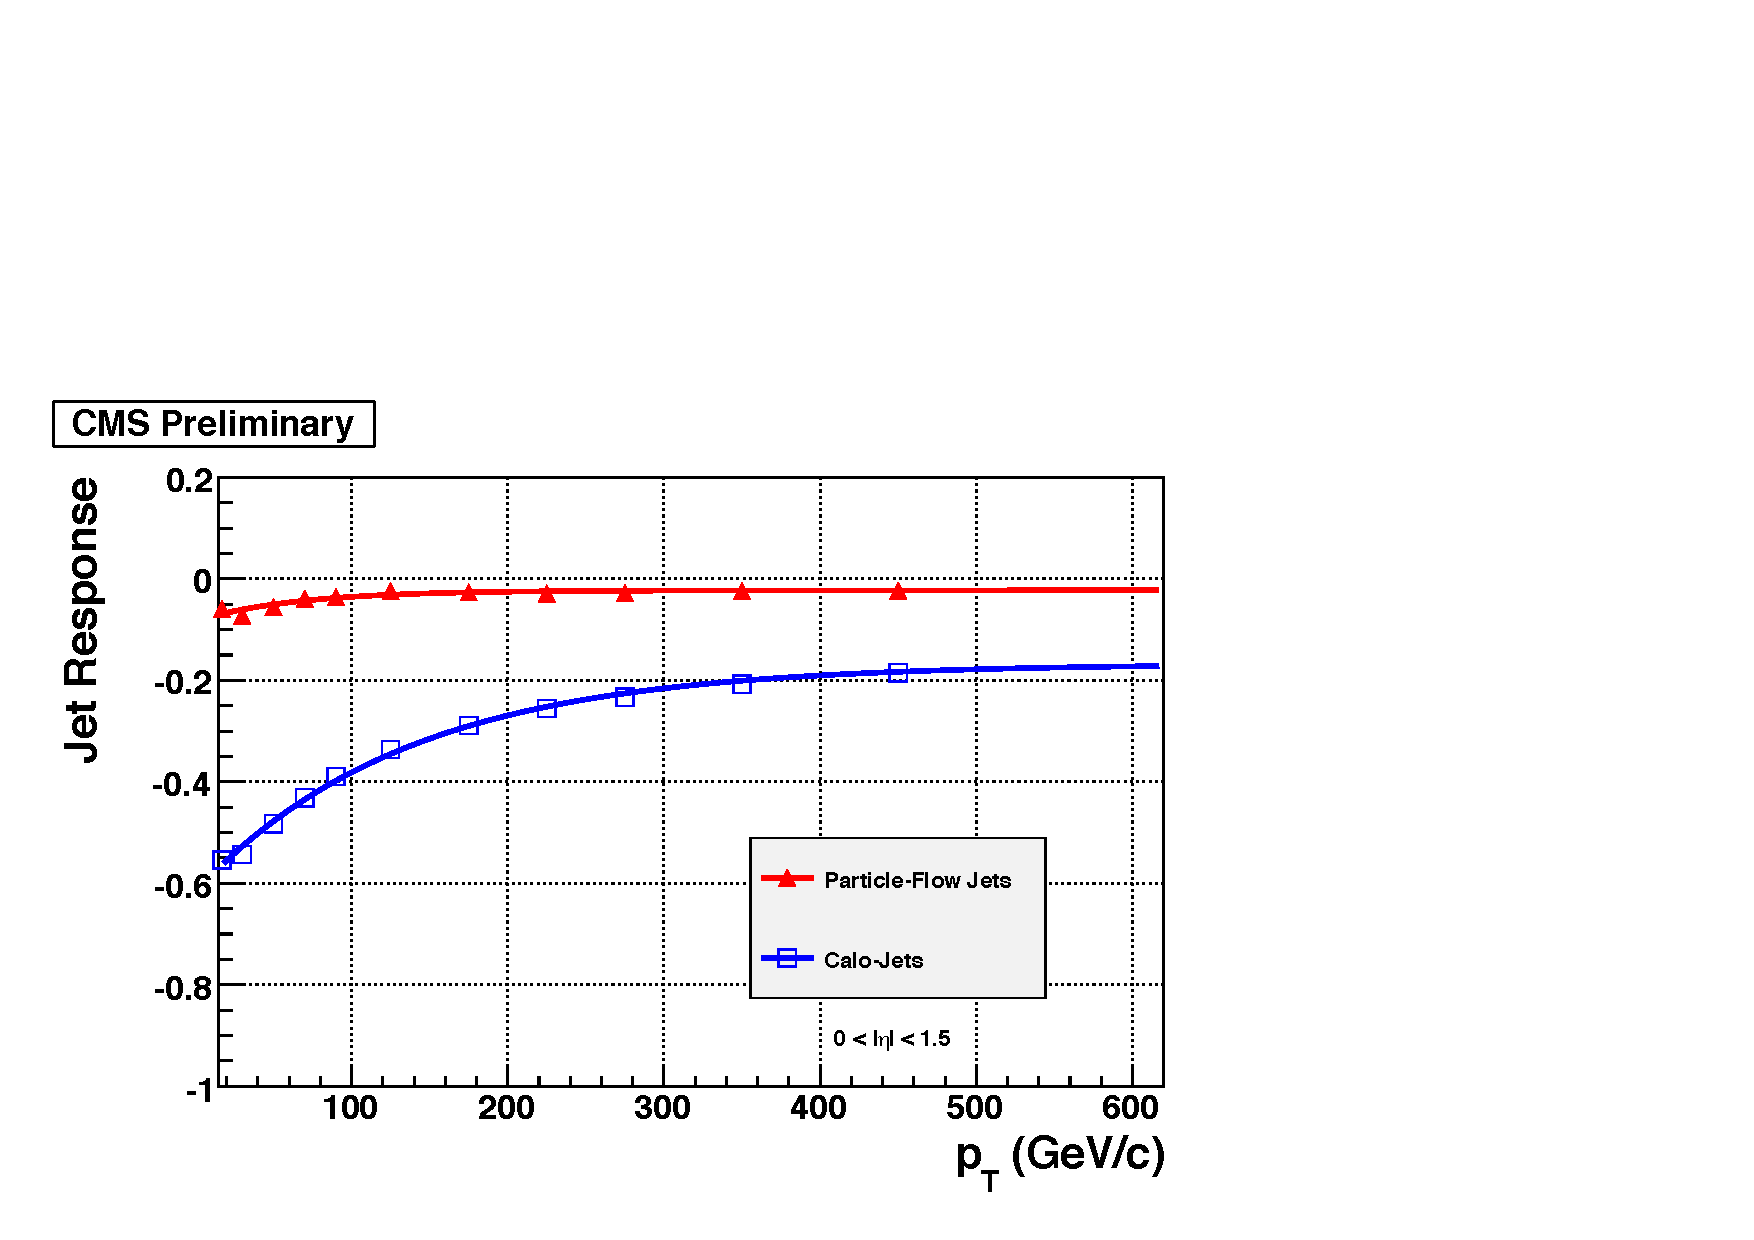
\includegraphics[width=\textwidth]{\figpath/Chapter3/Figure_008-b.pdf}
        \caption{}
        \label{fig:PFVsCaloJetResponse}
    \end{subfigure}
    \begin{subfigure}[t]{0.48\textwidth}
        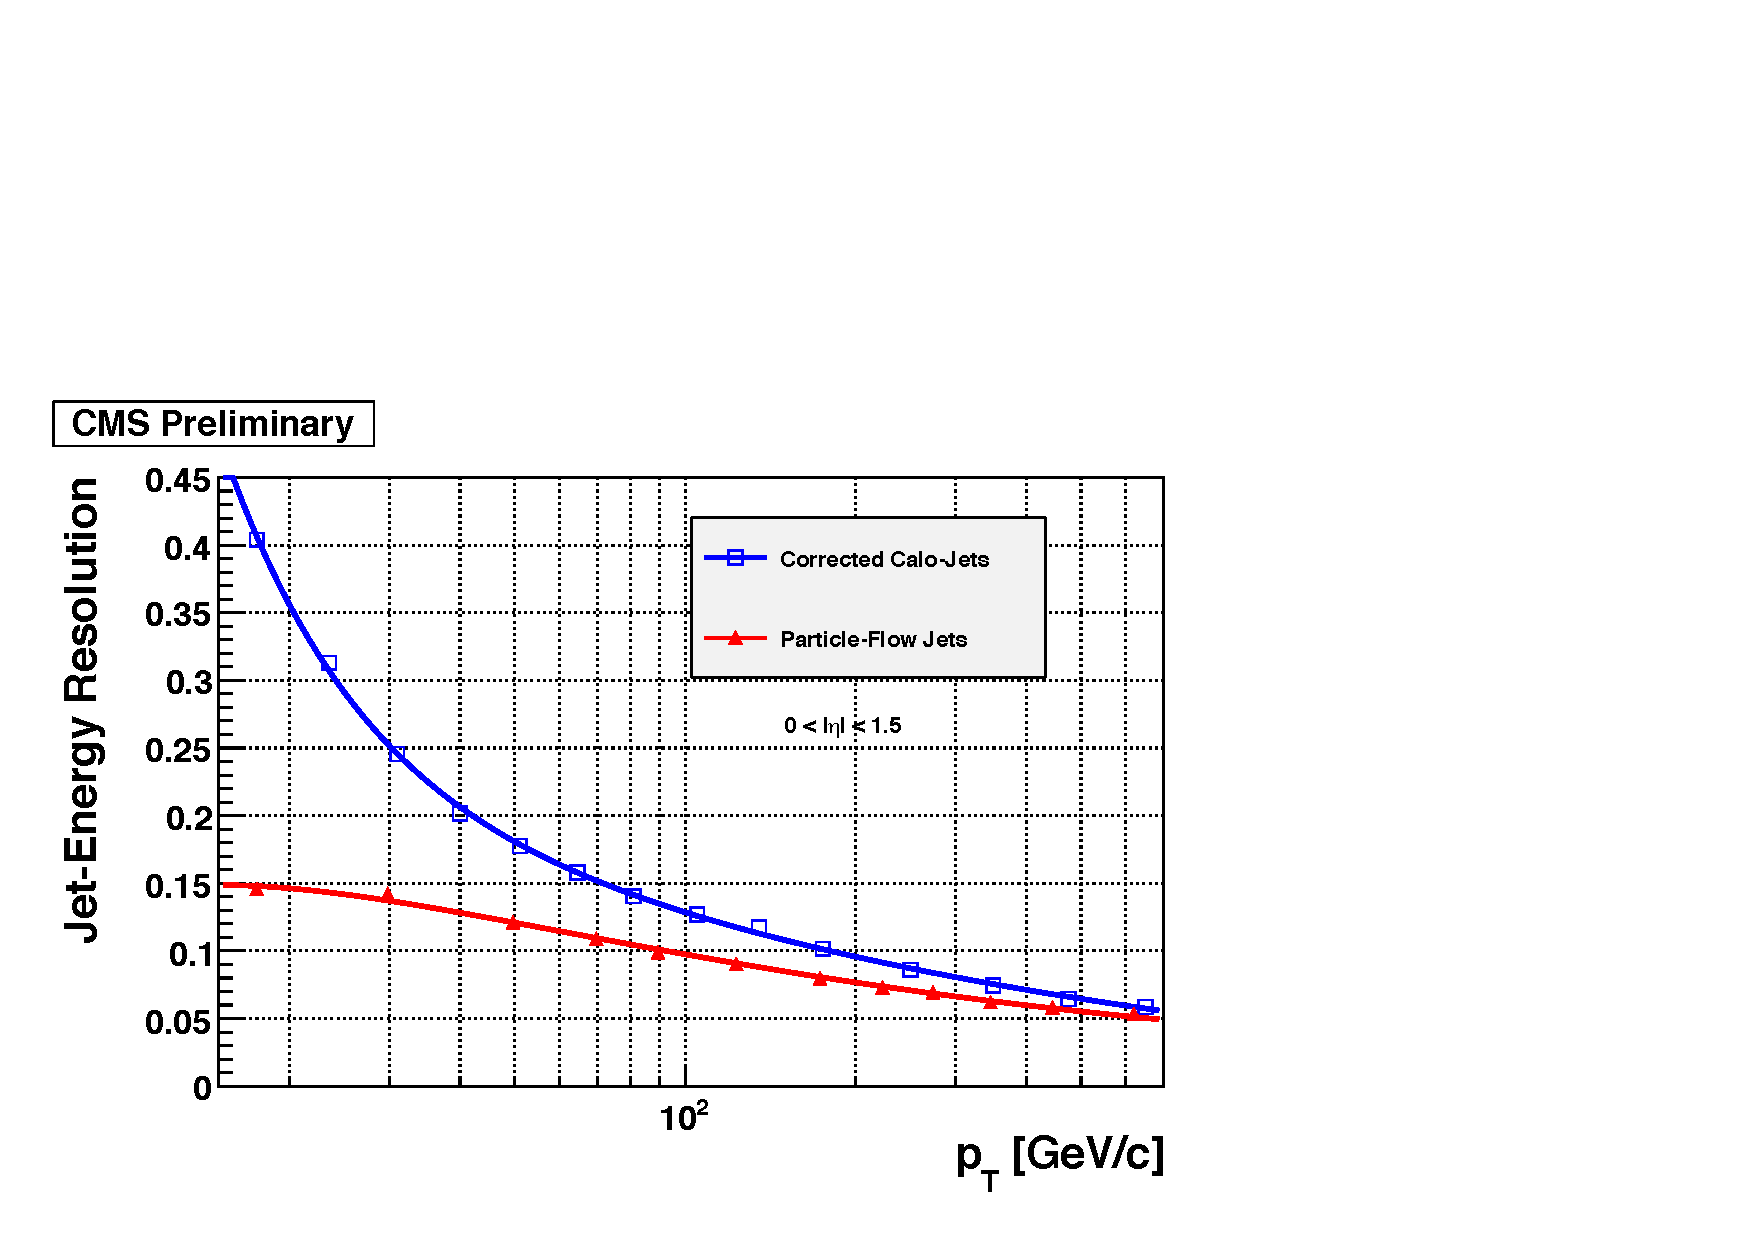
\includegraphics[width=\textwidth]{\figpath/Chapter3/Figure_010-a.pdf}
        \caption{}
        \label{fig:PFVsCaloJetResolution}
    \end{subfigure}
    \caption{Jet response (left) and resolution (right) as a function of \pt for jets made by clustering PF candidates and those clustering calorimeter towers. These figures were made using a MC sample with a center-of-mass energy of 10\tev, requiring the jets' \pt to be less than 750\gev, and that the jets are within \absetalt{1.5}~\cite{CMS-PAS-PFT-09-001}.}
\end{figure}

Before clustering the PF candidates, a pileup mitigation algorithm called charged hadron subtraction (CHS) is performed. As discussed in section~\ref{sec:tracks_and_vertices}, CMS can associate a track to a specific vertex. If these tracks are unambiguously associated to a pileup vertex, they are removed from the collection of PF candidates used to cluster jets and calculate the \VETslash. As shown in fig.~\ref{fig:PFJet_PileupComposition}, the CHS algorithm is able to remove about 50\% of the pileup energy produced during the same bunch crossing as the primary vertex. Any remaining energy from charged hadrons is coming from tracks that are not associated with a high quality vertex or which simply have too large a $\chi^{2}/N_{dof}$. Some of this is explained by the vertex reconstruction and identification inefficiency of about 30\%~\cite{Khachatryan:2198719}.

\begin{figure}[!hbt]
    \centering
    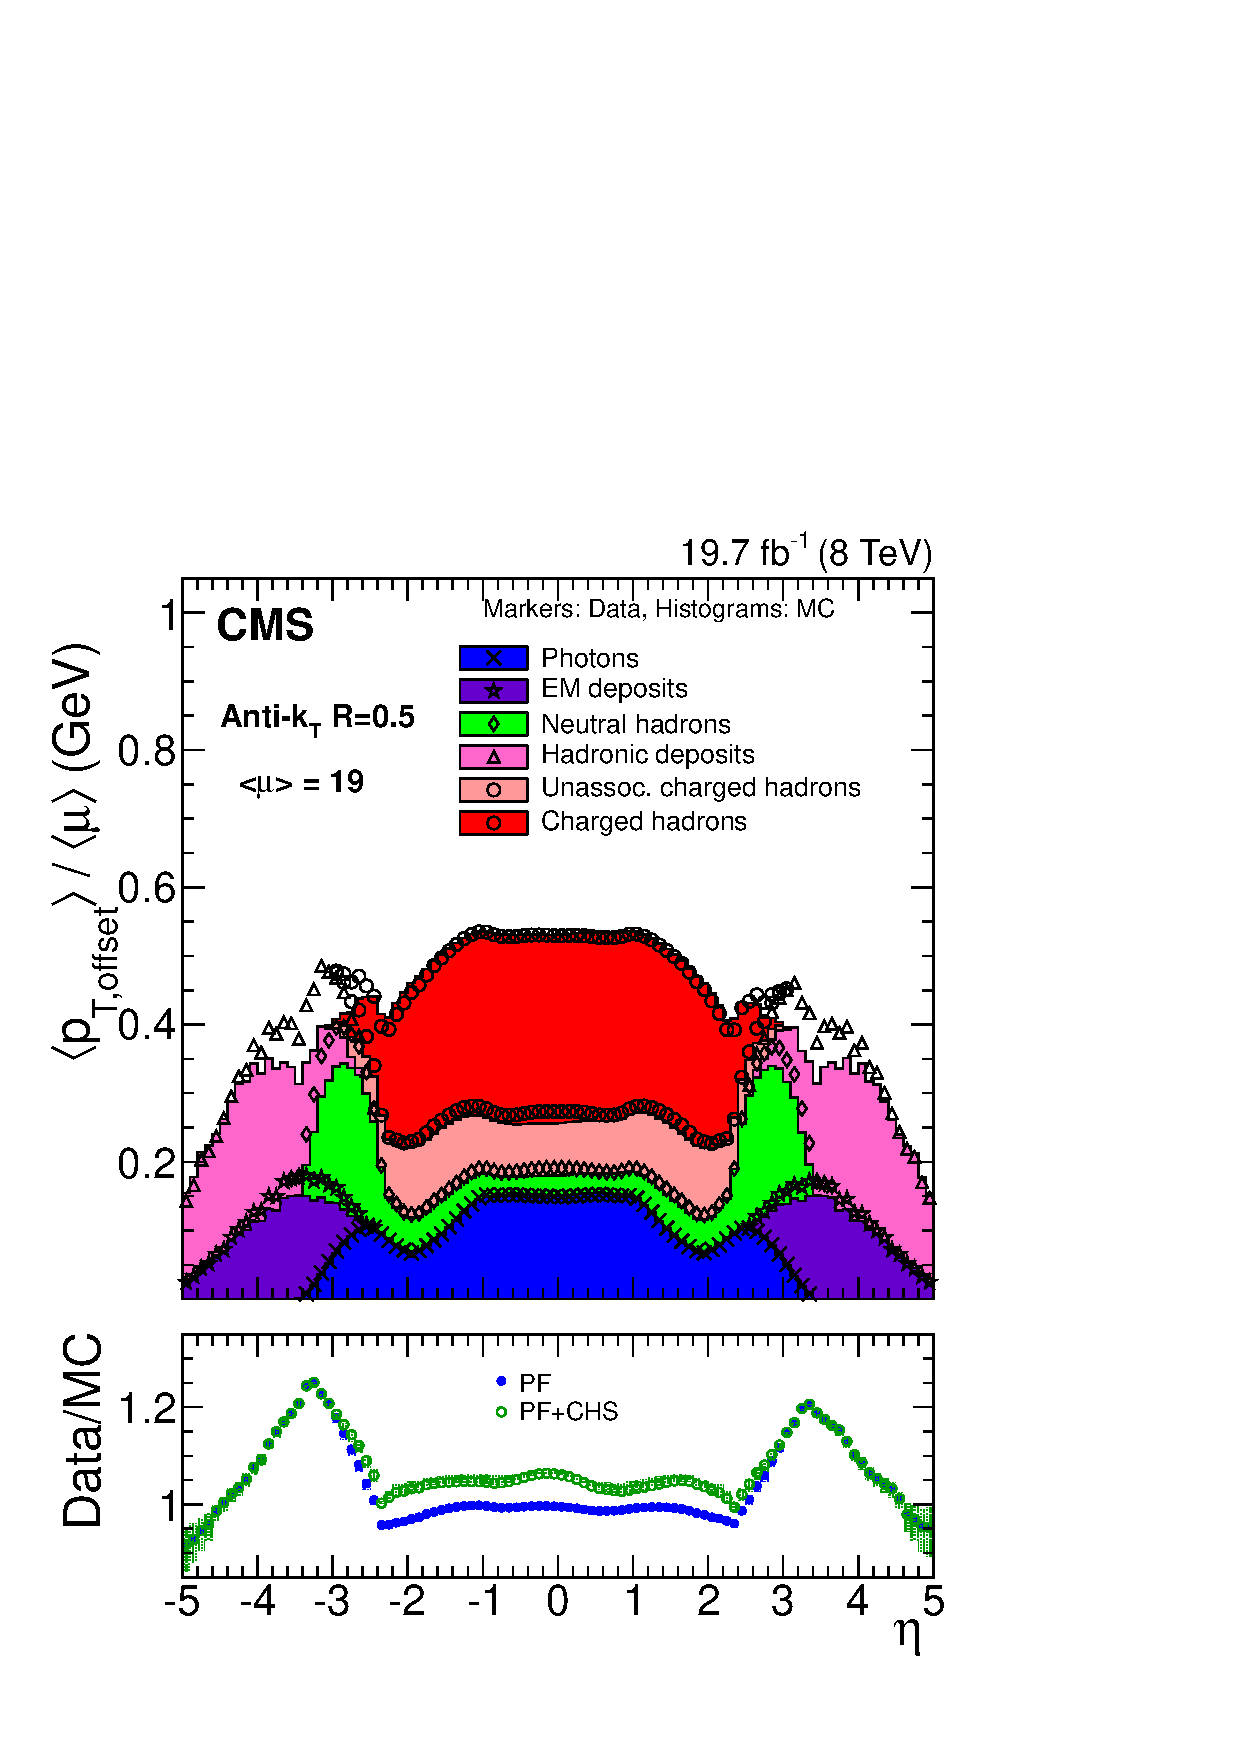
\includegraphics[width=0.95\textwidth]{\figpath/Chapter3/OffsetPerPU_Stacked_twopad_NPU-6_NPU-35.pdf}
    \caption{Pileup energy within a jet per additional proton-proton interaction ($\mu$) separated by type PF type. The fraction labeled ``charged hadrons'' will be removed by the CHS algorithm. The ratio of the data to the simulation is shown in the lower panel~\cite{Khachatryan:2198719}.}
    \label{fig:PFJet_PileupComposition}
\end{figure}

Like most other clustering algorithms (i.e. k\textsubscript{T}, Cambridge/Aachen, SisCone, etc.), anti-k\textsubscript{T} is iterative, wherein at each iteration two distance parameters are calculated.
$d_{ij}$ and $d_{iB}$, as defined in equation~\ref{eq:antikt_distance_parameter}, are the distance between two entities (PF candidates or existing cluster) and the distance from any one entity and the beam, respectively.
$y$ is the rapidity and R is a radius parameter, which is 0.5 in this analysis.
The anti-\textsubscript{T} algorithm is achieved when $p=-1$, whereas if $p=1$ ($p=0$) the k\textsubscript{T} (Cambridge/Aachen) algorithm is used instead.
If $d_{ij}<d_{iB}$, then entity $i$ and $j$ are combined vectorially.
However, if $d_{ij}>d_{iB}$, then entity $i$ is classified as a jet and is removed from further clustering.
This process continues until all PF candidates have been clustered~\cite{Cacciari:2008gp} and the momentum of the jet is the vectorial sum of all of the PF candidate momenta.
The result of this process can be seen in fig.~\ref{fig:anti-kT_jets}.

\begin{subequations}
    \label{eq:antikt_distance_parameter}
    \begin{align}
\label{eq:antikt_distance_parameter_1}d_{iB}={}&{p_{T}}_{i}^{2p}\\
\label{eq:antikt_distance_parameter_2}d_{ij}={}&min\left({p_{T}}_{i}^{2p},{p_{T}}_{j}^{2p}\right)\frac{\left(y_{i}-y_{j}\right)^{2}+\left(\varphi_{i}-\varphi_{j}\right)^{2}}{R^{2}}
    \end{align}
\end{subequations}

\begin{figure}[!hbt]
    \centering
    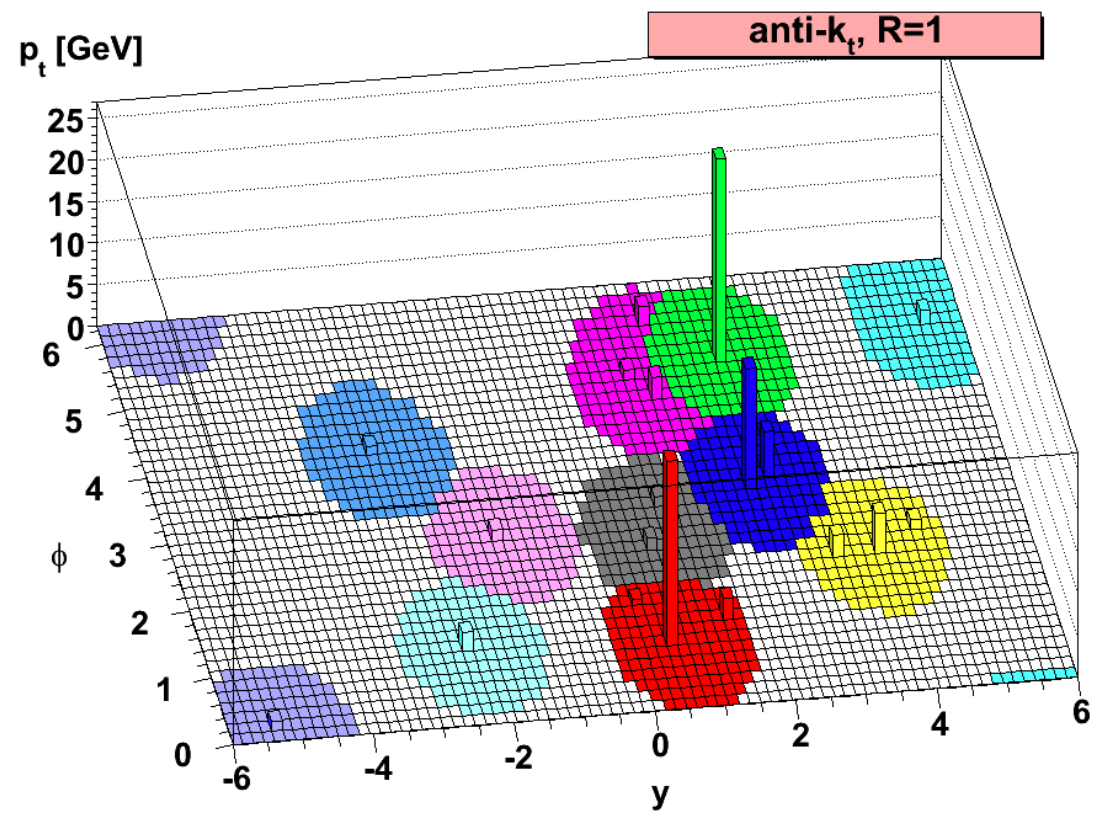
\includegraphics[width=0.95\textwidth]{\figpath/Chapter3/Anti-kT_Jets.png}
    \caption{Jets clustered from generator level partons using the anti-k\textsubscript{T} algorithm. This produces roughly circular jets with stable areas that are insensitive to additional soft particles~\cite{Cacciari:2008gp}.}
    \label{fig:anti-kT_jets}
\end{figure}

After CHS and clustering the momentum and energy of the jets still might not be the same as those from the initial parton, whether because of pileup or detector effects.
To correct for this, CMS uses a factorized approach, wherein each level of correction targets a specific effect and each correction is applied in order.
The goal is to make sure each jet has a relative response ($RelRsp=\frac{\ptsup{reco}}{\ptsup{gen}}$) of 1.
This type of scaling is commonly referred to as a jet energy correction (JEC)\footnote{The terms \pt and energy will be used interchangeably only when discussing the jet energy corrections. This is because the corrections will affect both the energy and \pt terms within the jet 4-momentum.}.
The first level of correction, commonly referred to as the L1FastJet corrections, starts by removing any remaining pileup\footnote{CHS was able to remove pileup energy coming from charged hadrons, but not energy added to the jet from, for example, neutral hadrons or photons as seen in figure~\ref{fig:PFJet_PileupComposition}.} or electronic noise energy that may have made it into the jet reconstruction.
This multiplicative correction will only remove energy from within the jet and will take the form in equation~\ref{eq:JEC_L1FastJet}, where $\rho$ is the median energy density of the event, $A$ is the jet area, and $f$ is an estimate of the offset inside the jet per unit of jet area~\cite{JINST2011,Cacciari2007}.
\begin{equation}
\label{eq:JEC_L1FastJet}
\ptsup{L1Corrected}=\ptsup{uncorrected}\cdot\left(1-A\frac{f\left(\eta,\rho,A\right)}{\ptsup{uncorrected}}\right)
\end{equation}
The L2Relative correction seeks to correct for the non-linearity in the jet response as a function of $\eta$ while the L3Absolute correction does the same thing as a function of \pt.
These are again multiplicative corrections that can either increase or decrease the energy of the jet.
All three corrections are applied to both data and simulation.
An additional level of correction, termed L2L3Residual, is applied only to data to correct for the difference in scale between the data and simulation. For a more in-depth discussion of pileup mitigation techniques and jet energy corrections see appendix~\ref{appendix:JERC}.

A set of quality cuts, collectively called PF jet identification, are applied to the resulting collection of jets to ensure that only real, hard scatter PF jets are used during the analysis~\cite{CMS-AN-2010-003}. Several working points are defined at varying levels of efficiency and purity, but this analysis makes use of the loose criteria shown in table~\ref{tab:PFJetID}~\cite{PFJetID}. The variables used in these cuts include the fraction of neutral hadrons in the jet $f_{NH}$, the fraction of neutral EM particles $f_{\gamma}$, the fraction of charged hadrons $f_{CH}$, the fraction of charged EM particles $f_{EM}$, the number of constituents $n_{constituents}$, and the multiplicity of charged particles $n_{charged}$. In addition to the PF jet quality cuts, this analysis requires that all jets be within \abseta{2.4}, the leading jet have $\pt>30\gev$, and all other jets have $\pt>25\gev$. Additionally, all jets are required to be at least ${\Delta}R(\textrm{jet},\textrm{lepton})>0.3$ away from any isolated, selected lepton.
\begin{table}[htbp]
    \caption{Cut based PF jet identification requirements for the loose working point.}
    \centering
    \begin{tabular}{ll}
        \hline
        \multirow{2}{*}{Cut Variable}               & Cut Value \\\cline{2-2}
                                                    & Loose \\
        \hline
        $f_{CH}>$                                  & 0.0        \\
        $f_{NH}<$                                  & 0.99 \\
        $f_{\gamma}<$                              & 0.99        \\
        $f_{EM}<$                                  & 0.99         \\
        $n_{charged}>$                              & 0          \\
        $n_{constituents}>$                         & 1           \\
        \hline
    \end{tabular}
    \label{tab:PFJetID}
\end{table}

\section{b-tagging}
\label{sec:btagging}

Bottom quarks are interesting because they are often associated with the decays of the top quark and the Higgs boson.
The experimental signature of a hadronizing bottom quark will be a \textit{b-jet}.
This flavor of jet is identifiable because of the unique decay kinematics of b hadrons, including their long lifetime (1.5\unit{ps}$\Rightarrow{c}\tau\approx450\mum$) and high \pt decay products~\cite{Olive:2016xmw,PhysRevD.17.171}.
Additionally, b hadrons have a relatively large mass ($\sim5\gev$), which means they have a higher track multiplicity than other quark jets, about 5 on average.
The displaced tracks will form a secondary vertex with a large impact parameter which can be measured by the tracking sub-detector.
CMS uses the Combined Secondary Vertex (CSV) algorithm to tag jets as either being initiated by a bottom quark or some other parton (u, d, s, c, and g)~\cite{Weiser:927399,BTV-12-001}.

In order to identify secondary vertices, the algorithm starts from a subset of well-reconstructed tracks.
These tracks must have a \pt greater than 1\gev, $\chi^{2}/N_{dof}<5$, a transverse (longitudinal) impact parameter less than 0.2\unit{cm} (17]\unit{cm}), and a $\Delta{R}$ to the jet axis less than 0.3.
Each track is also required to have at least 8 hits in the tracker, of which 2 must be from the pixel detector.
To reduce the effects of pileup the track's distance of closest approach to the jet axis (primary vertex) must be less than 700\mum (5\unit{cm}).
Once the tracks are selected, the secondary vertices are reconstructed using the AVF described in section~\ref{sec:tracks_and_vertices}.
At each iteration, if the track weight is greater than 0.5 the track is removed and the iterations continue until no more secondary vertices are found.
In order to increase the purity of the secondary vertices they are required to share no more than 65\% of their tracks with the primary vertex, to be more then $3\sigma$ away from the primary vertex in the $\eta-\varphi$ plane, and the $\Delta{R}$ between the vertex and the jet direction must be less than 0.5.
A secondary vertex candidate is also rejected is its radial distance to the primary vertex is greater than 2.5\unit{cm} and its invariant mass is close to that of the \PKz.
The jets are then assigned as being associated to a real secondary vertex, a \textit{pseudo-vertex}, or no vertex.
A \textit{pseudo-vertex} if created when the AVF fails to find a secondary vertex, but there are at least two tracks with $S_{ip}>2$, where $S_{ip}$ is the significance of the track's impact parameter defined as the value of the impact parameter divided by its uncertainty.

The following are used as inputs to the CSV tagger:
\begin{itemize}
    \item The significance of the flight distance in the transverse plane between the secondary and primary vertices.
    \item The invariant mass of the secondary vertex (the mass of all of the tracks associated with that vertex).
    \item The number of tracks associated to the secondary vertex.
    \item The ratio of the energy carried by the tracks associated to the secondary vertex and all tracks in the jet.
    \item The $\Delta\eta$ between the jet axis and the tracks associated to the secondary vertex.
    \item The transverse impact parameter significance of the tracks which raises the invariant mass above 1.5\gev, the charm threshold. The tracks are ordered by decreasing significance and combined one-by-one until the charm threshold is met.
    \item The number of tracks in the jet.
    \item The three-dimensional impact parameter significance of each track.
    \item The secondary vertex category (real, pseudo, or none).
\end{itemize}
All of the inputs are computed for jets with at least one associated real secondary vertex. The first input is not computed for jets with only a \textit{pseudo-vertex} because it doesn't have a well-defined position. Only the last three inputs, which are track based, are computed when no secondary vertex is found for the jet.

The inputs to the algorithm are combined using a likelihood-based discriminator, where the likelihood is defined in equation~\ref{eq:csv_likelihood}.
\begin{equation}
\label{eq:csv_likelihood}
\mathcal{L}^{b,c,q}=f^{b,c,q}\left(\alpha\right)\times\prod_{i}f_{\alpha}^{b,c,q}\left(x_{i}\right)
\end{equation}
Here $b$,$c$, and $q=\left\{u,d,s,q\right\}$ are the flavor of jet, $\alpha$ is the vertex category, $f^{b,c,q}\left(\alpha\right)$ is the probability density function (PDF) for the jet of a given flavor to have a vertex of category $\alpha$, $x_{i}$ is one of the inputs, and $f_{\alpha}^{b,c,q}\left(x_{i}\right)$ is the PDF for $x_{i}$ given the jet flavor and vertex category. The discriminator is then defined in equation~\ref{eq:csv_discriminator}.
\begin{equation}
\label{eq:csv_discriminator}
d_{CSV}=f_{BG}\left(c\right)\frac{\mathcal{L}^{b}}{\mathcal{L}^{b}+\mathcal{L}^{c}}+f_{BG}\left(q\right)\frac{\mathcal{L}^{b}}{\mathcal{L}^{b}+\mathcal{L}^{q}}
\end{equation}
In this case, $f_{BG}\left(c\right)=0.25$ and $f_{BG}\left(q\right)=0.75$ are weights that approximate the expected background (BG)composition.

Working points for this discriminator are defined using probability to mis-identify a light quark or gluon jet as a b-jet~\cite{CMS-PAS-BTV-13-001}.
The loose, medium, and tight working points have a 10\%, 1\%, and 0.1\% mistag rate, respectively. 
This analysis uses the medium working point ($d_{CSV}>0.679$), which has a tagging efficiency of $\geq60\%$ as shown in fig.~\ref{fig:bDiscriminator_efficiency}.
For example, a b-jet with a \pt of 80\gev has a tagging efficiency of 75\%
Fig.~\ref{fig:bDiscriminator} shows the CSV discriminator distribution in both a QCD dominated and \ttbar dominated sample.
The MC simulation is separated by jet flavor to show the discrimination power of the CSV algorithm.
\begin{figure}[!hbt]
    \centering
    \begin{subfigure}[t]{0.48\textwidth}
        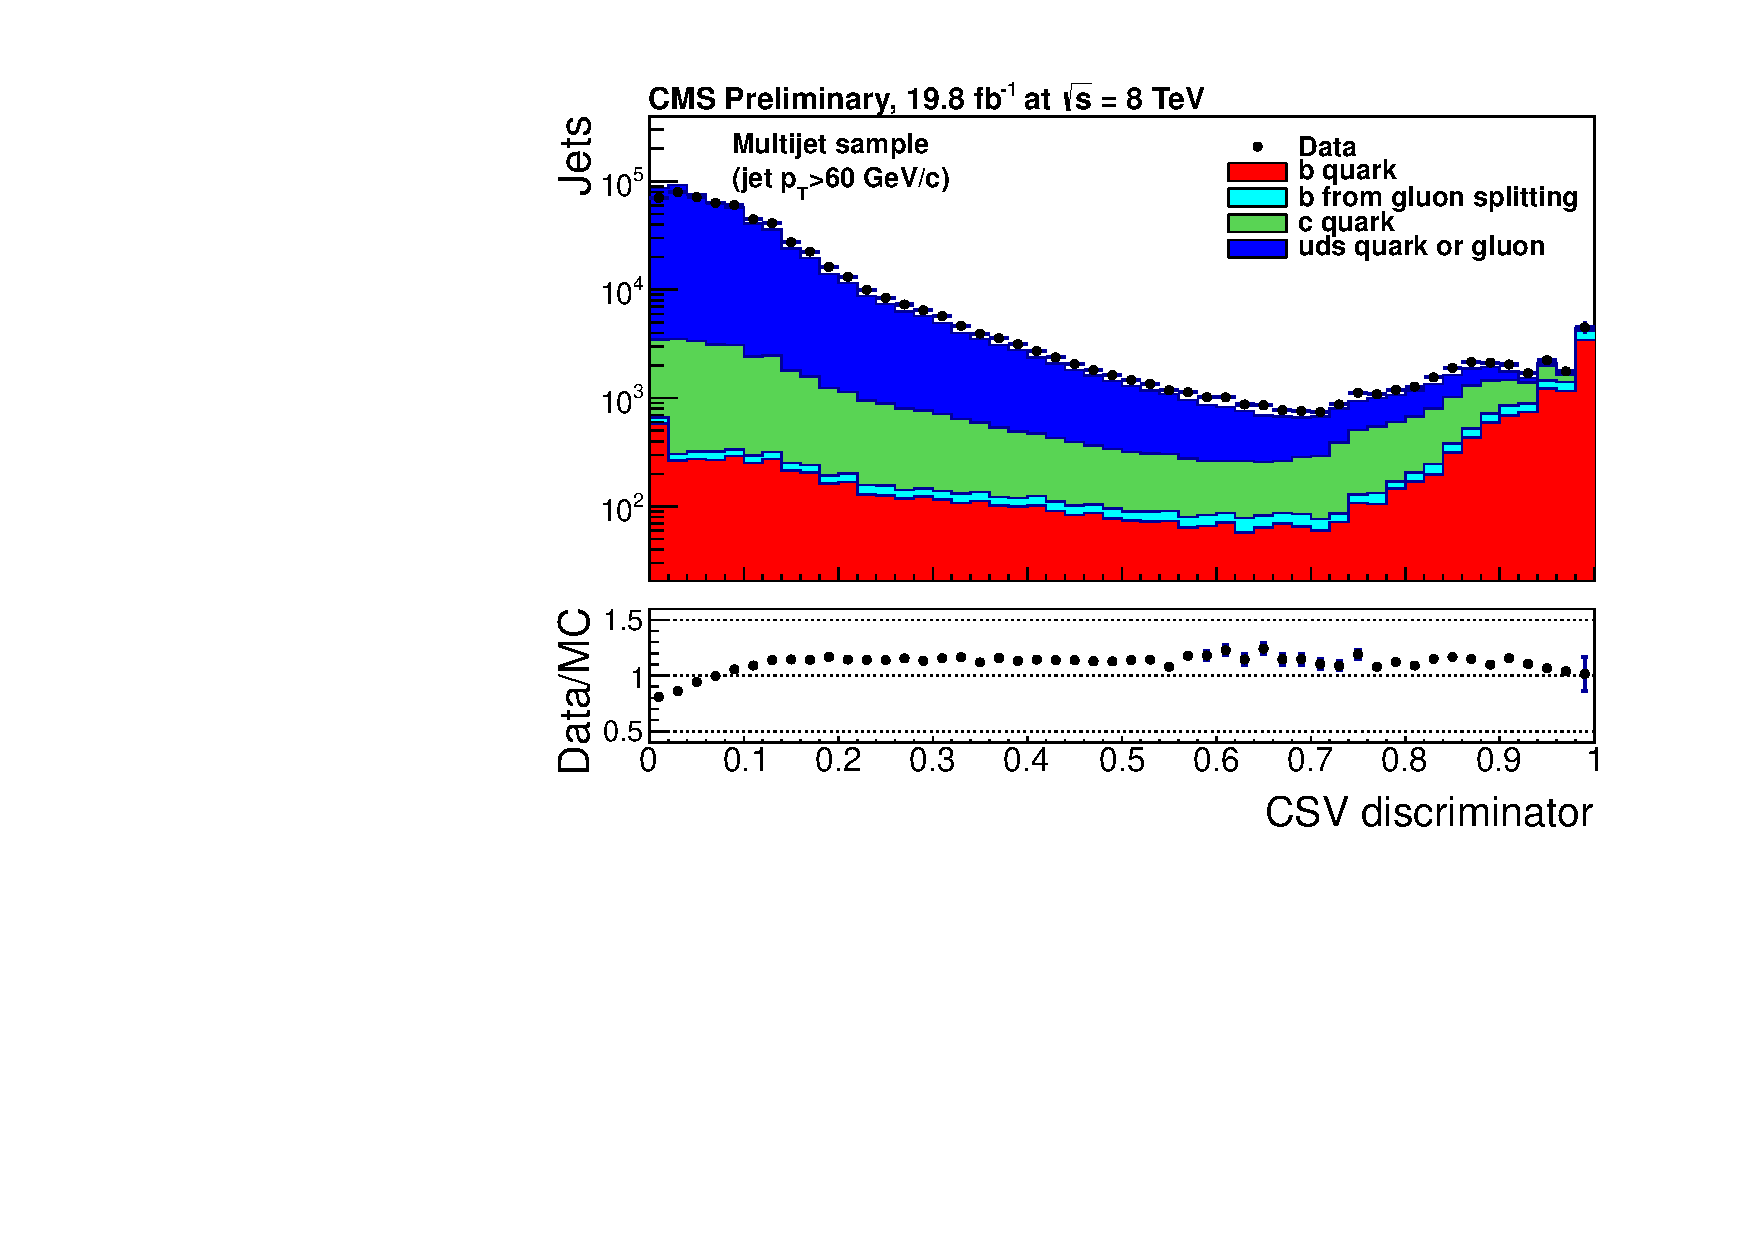
\includegraphics[width=\textwidth]{\figpath/Chapter3/b-tagging/Figure_006-e.pdf}
        \caption{}
        \label{fig:bDiscriminator_QCD}
    \end{subfigure}
    \begin{subfigure}[t]{0.48\textwidth}
        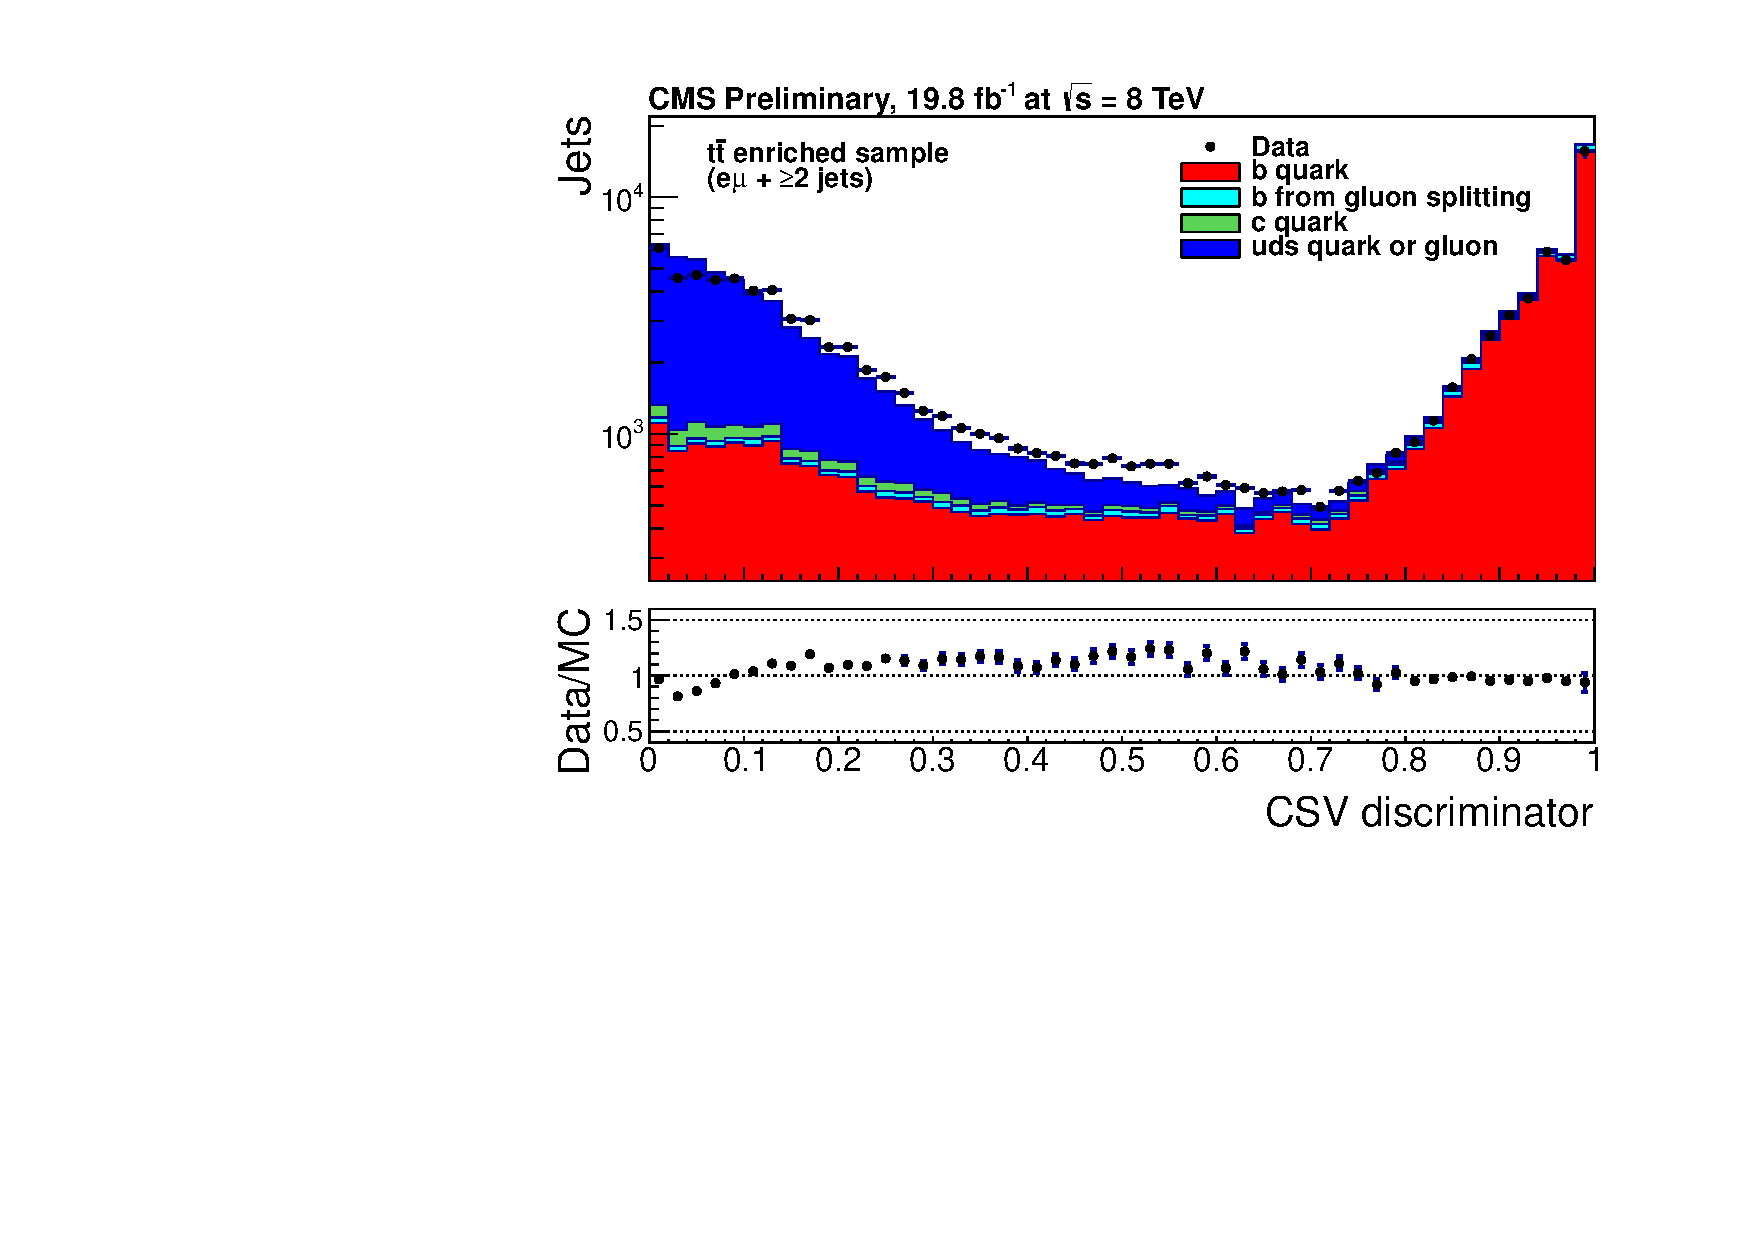
\includegraphics[width=\textwidth]{\figpath/Chapter3/b-tagging/Figure_006-f.pdf}
        \caption{}
        \label{fig:bDiscriminator_ttbar}
    \end{subfigure}
    \caption{The $d_{CSV}$ distribution in a (left) QCD dominated sample and (right) a \ttbar dominated sample~\cite{CMS-PAS-BTV-13-001}.}
    \label{fig:bDiscriminator}
\end{figure}

\begin{figure}[!hbt]
    \centering
    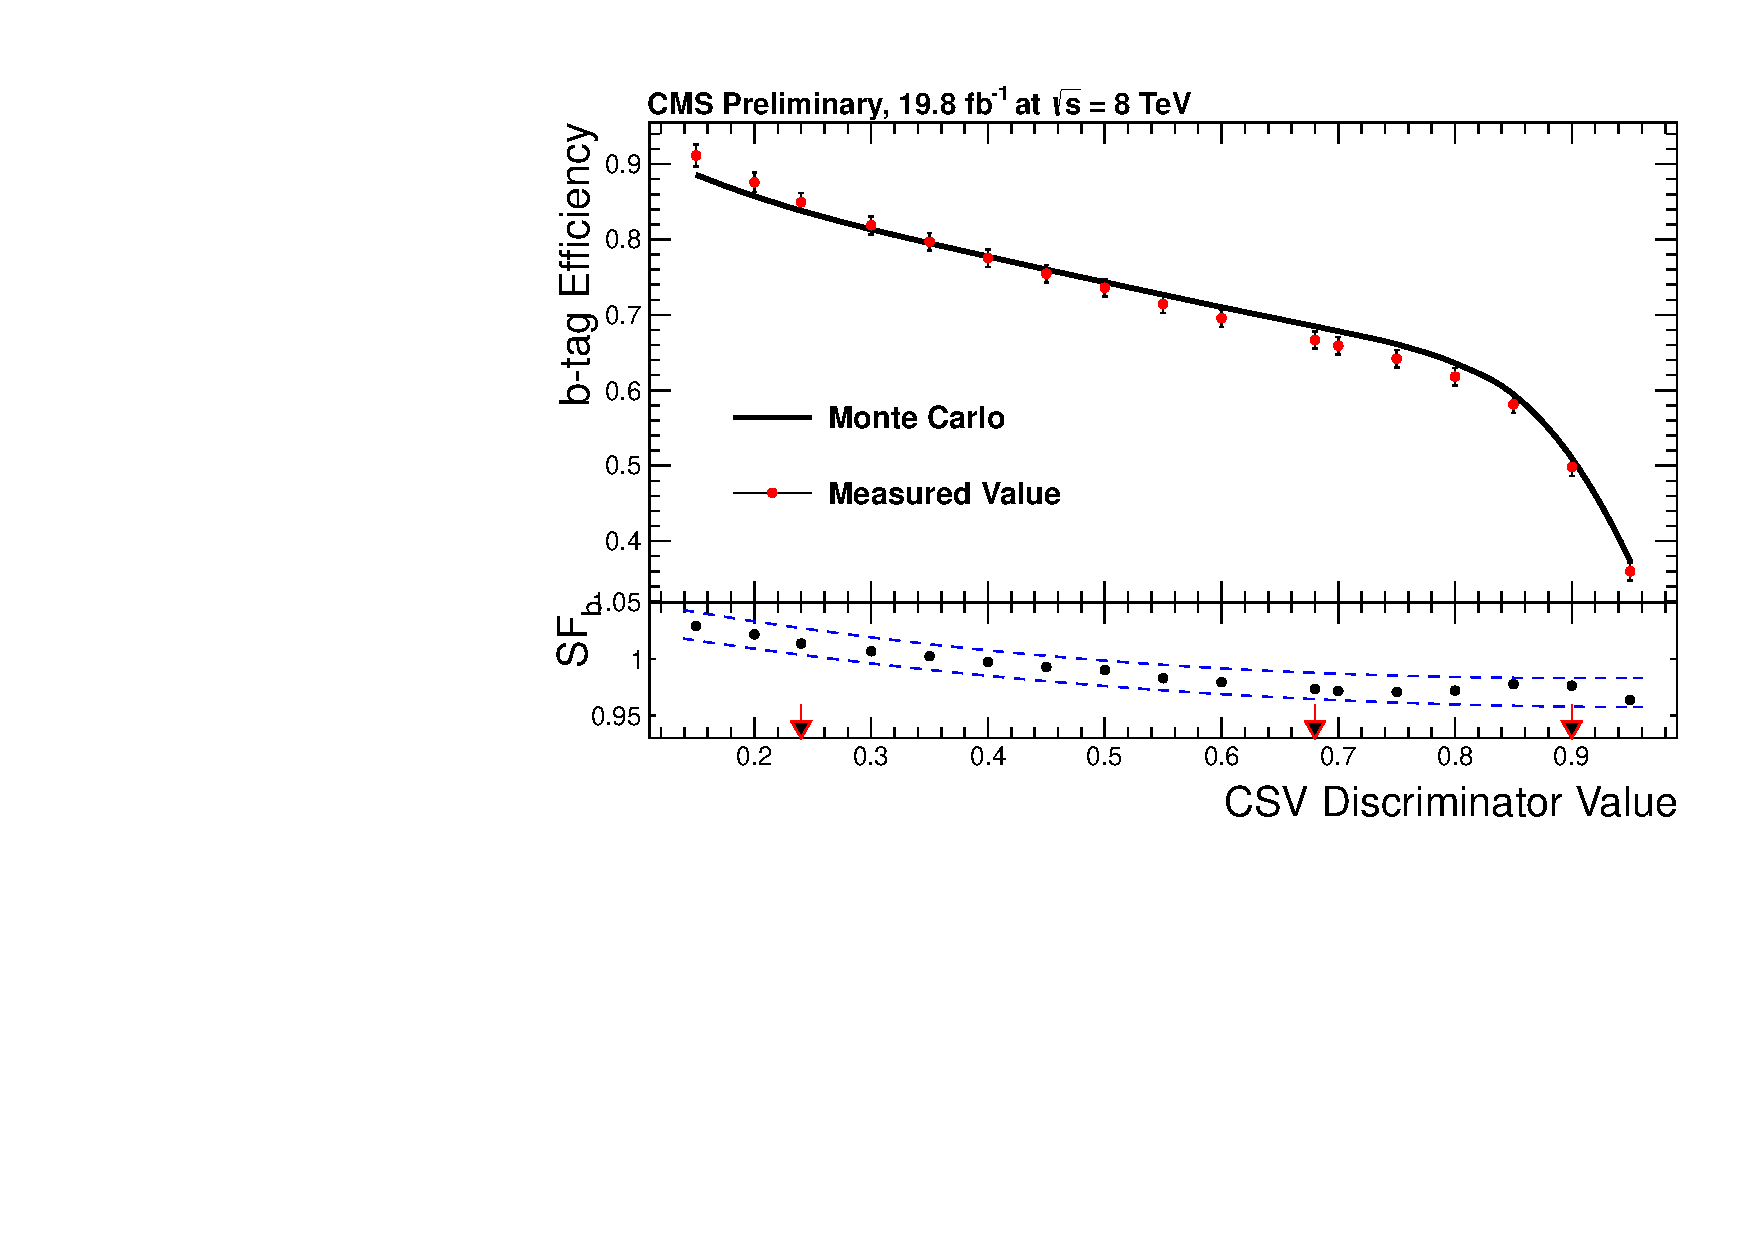
\includegraphics[width=0.95\textwidth]{\figpath/Chapter3/b-tagging/Figure_012-b.pdf}
    \caption{The b-tagging efficiency as a function of the CSV discriminator ($d_{CSV}$) value for both data and MC. The lower panel shows the ratio of the data and MC efficiencies and the arrows along the $x$-axis show the loose, medium, and tight working point values~\cite{CMS-PAS-BTV-13-001}.}
    \label{fig:bDiscriminator_efficiency}
\end{figure}

\section{Missing Transverse Energy}
\label{sec:MET}
%https://twiki.cern.ch/twiki/bin/view/CMSPublic/WorkBookMetAnalysis

While CMS is designed to detect as many particles as possible, some particles may be outside of the detector acceptance, may be mis-measured, or may simple not interact with the detection elements.
Examples of this are a particle which is beyond and $\eta$ of 5.0 or a neutrino, which will make it through the detector without ever interacting or a BSM particle which do not interact with the detector.
Furthermore, there may be additional particles in the event due to pileup which can can lead to fake \VETslash due to calorimeter thresholds and response nonlinearities.
Because the proton beams have near zero momentum in the $x$ and $y$ directions, only traveling in the $z$ direction, any imbalance in the momentum in the transverse plane indicates additional, missing, or mis-measured particles.
This imbalance is called missing transverse momentum and is the negative vector sum of \ptvec for all PF candidates in the event as seen in equation~\ref{eq:MET_uncorr_simple}.
The magnitude of this quantity is known as missing transverse energy and is represented as \ETslash~\cite{METperf2012}. A schematic of these two quantities is shown in fig.~\ref{fig:MET_schematic}.
\begin{equation}
\label{eq:MET_uncorr_simple}
\VETslashUncorr=-\sum_{i}{\vec{p}_{T}}^{\text{ }i}
\end{equation}

\begin{figure}[!hbt]
    \vspace*{-0.5cm}
    \centering
    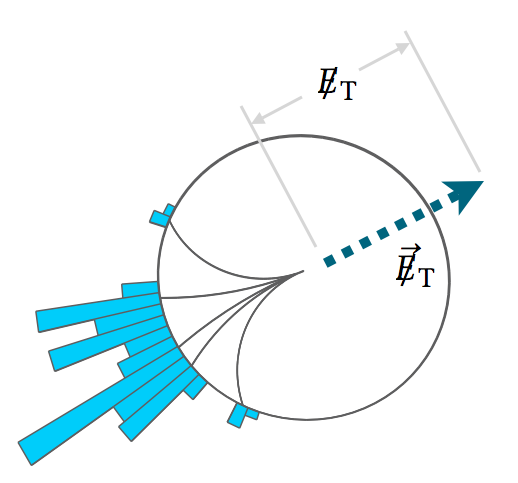
\includegraphics[width=0.95\textwidth]{\figpath/Chapter3/tai_20120616_met_schematic.png}
    \caption{A schematic of the \VETslash and \ETslash quantities~\cite{METAnalysis}.}
    \label{fig:MET_schematic}
\end{figure}

Because the \VETslash is affected by every \textit{visible} particle in the event, meaning particles which interact using the electromagnetic or strong forces, it is particularly sensitive to minimum energy thresholds in the calorimeters, inefficiencies and \pt thresholds in the tracker, and the non-linear, non-compensating response of the ECAL and HCAL.
While electrons and muons have a very good resolution and are typically measured correctly, composite objects like jets have a non-negligible affect on the \VETslash and the bias due to these effects can be reduced by correcting the jets and propagating those corrections to the \VETslash.
Unfortunately the corrections discussed in section~\ref{sec:jets} are applied to the composite object and not the the individual constituents\footnote{A method which is being actively worked on.}.
The jet energy corrections are therefore propagated to the \VETslash with the requirements that $f_{EM}<0.9$ and $\pt>10\gev$ so as to exclude electrons which may sometimes produce a non-genuine jet.
This type of correction is called Type-1 corrected \VETslash and is what is used in this analysis as a proxy for the undetected neutrino coming from the decay of one of the W boson.
%https://twiki.cern.ch/twiki/bin/view/CMS/METType1Type2Formulae
\begin{subequations}
    \label{eq:MET_type1}
    \begin{align}
\VETslashUncorr={}&-\sum_{i \in \textrm{jets}}\ptvecsub{i}-\sum_{i \notin \textrm{jets}}\ptvecsub{i} \label{eq:MET_uncorr_PFObjects}\\
={}&-\sum_{\textrm{jet}}\ptvecsubsup{jet}{uncorr.}-\sum_{i \notin \textrm{jets}}\ptvecsub{i} \label{eq:MET_uncorr_PFObjects_jets} \\
={}&-\sum_{\substack{\textrm{jet} \\ \ptvecsubsup{jet}{L123} > 10 \gev}}\ptvecsubsup{jet}{uncorr.}-\sum_{\substack{\textrm{jet} \\ \ptvecsubsup{jet}{L123} < 10 \gev}}\ptvecsubsup{jet}{uncorr.}-\sum_{i \notin \textrm{jets}}\ptvecsub{i} \label{eq:MET_uncorr_threshold}\\
\begin{split}\label{eq:MET_uncorr}
={}&-\sum_{\substack{\textrm{jet} \\ \ptvecsubsup{jet}{L123} > 10 \gev}}\ptvecsubsup{jet}{L1}-\sum_{\substack{\textrm{jet} \\ \ptvecsubsup{jet}{L123} > 10 \gev}}\left(\ptvecsubsup{jet}{uncorr.}-\ptvecsubsup{jet}{L1}\right)\\
&-\sum_{\substack{\textrm{jet} \\ \ptvecsubsup{jet}{L123} < 10 \gev}}\ptvecsubsup{jet}{uncorr.}-\sum_{i \notin \textrm{jets}}\ptvecsub{i}
\end{split}\\
\begin{split}\label{eq:MET_type1_final}
\VETslashsup{Type-1}={}&-\sum_{\substack{\textrm{jet} \\ \ptvecsubsup{jet}{L123} > 10 \gev}}\ptvecsubsup{jet}{L123}-\sum_{\substack{\textrm{jet} \\ \ptvecsubsup{jet}{L123} > 10 \gev}}\left(\ptvecsubsup{jet}{uncorr.}-\ptvecsubsup{jet}{L1}\right) \\
&-\sum_{\substack{\textrm{jet} \\ \ptvecsubsup{jet}{L123} < 10 \gev}}\ptvecsubsup{jet}{uncorr.}-\sum_{i \notin \textrm{jets}}\ptvecsub{i}
\end{split}
    \end{align}
\end{subequations}

Equation~\ref{eq:MET_uncorr_simple} shows the simplified and uncorrected model of \VETslash which can be broken into two categories, those particles which are contained in jets and those which are not.
This is shown in equation~\ref{eq:MET_uncorr_PFObjects}, but can be simplified further to equation~\ref{eq:MET_uncorr_PFObjects_jets} by noting that the first term is simply the sum of \pt for the uncorrected jets.
In equation~\ref{eq:MET_uncorr_threshold} the jets are further broken into two classes based on their corrected \pt and in equation~\ref{eq:MET_uncorr} the jets are broken into the pileup corrected jets term and a term for the pileup itself, where $\left(\ptvecsubsup{jet}{uncorr.}-\ptvecsubsup{jet}{L1}\right)$ is the additional energy due to pileup (offset).
Now that the \VETslash is fully broken down it can be corrected by replacing $\ptvecsubsup{jet}{L1}$ in the first term with $\ptvecsubsup{jet}{L123}$ to give equation~\ref{eq:MET_type1_final}.
This is a correction on the clustered energy in the event above a given threshold~\cite{METAnalysis}.
In this analysis the resulting quantity is required to have at least 25\gev in order to reduce the QCD events making it through the selection process.


In addition to propagating the JEC to the \VETslash, CMS also filters events and or \VETslash contribution which might introduce noise from the calorimeters or beam halo~\cite{METperf2011}. An additional modification to the \VETslash to correct a $\varphi$ asymmetry is also used, but will be discussed further in section~\ref{sec:met_phi_corrections}. A pileup correction to the \VETslash was also available, but was not implemented in this analysis. It is nevertheless discussed in appendix~\ref{appendix:MET}.

\section{Event Generation}
\label{sec:event_generation}

In the search for new physics, a signal will generally appear as a small deviation from the SM prediction.
In order to disentangle the SM background from a rare signal the SM and new physics prediction must be extremely accurate.
The predictions are samples made by Monte Carlo (MC) event generators which are broken up by physics process and final state and then recombined during the analysis~\cite{Siegert:2010cru,Mangano:2005dj,Dobbs:2004qw}.
These generators are able to simulate a full event (bunch crossing) at the parton level, which is nicely illustrated in fig.~\ref{fig:ttH_event}.
The image shows a $t\bar{t}h$ final state including final state gluons (QCD) and hadronization.
While the entire event from hard scatter production to hadronization cannot be described using perturbation theory, the hard process can be calculated using fixed order perturbation theory and matrix elements (ME).
The parton showers, red lines in fig.~\ref{fig:ttH_event}, then connect the hard process with the hadronization scale.
Phenomenological models are used to simulate the hadronization into stable particles and the underlying event (UE), which is the usually softer interactions by the constituents of the protons which did not take part in the hard scatter process.
Photon and gluon emission from the initial protons and final state partons, respectively called initial state radiation (ISR) and final state radiation (FSR), must also be simulated.

\begin{figure}[!hbt]
    \vspace*{-0.5cm}
    \centering
    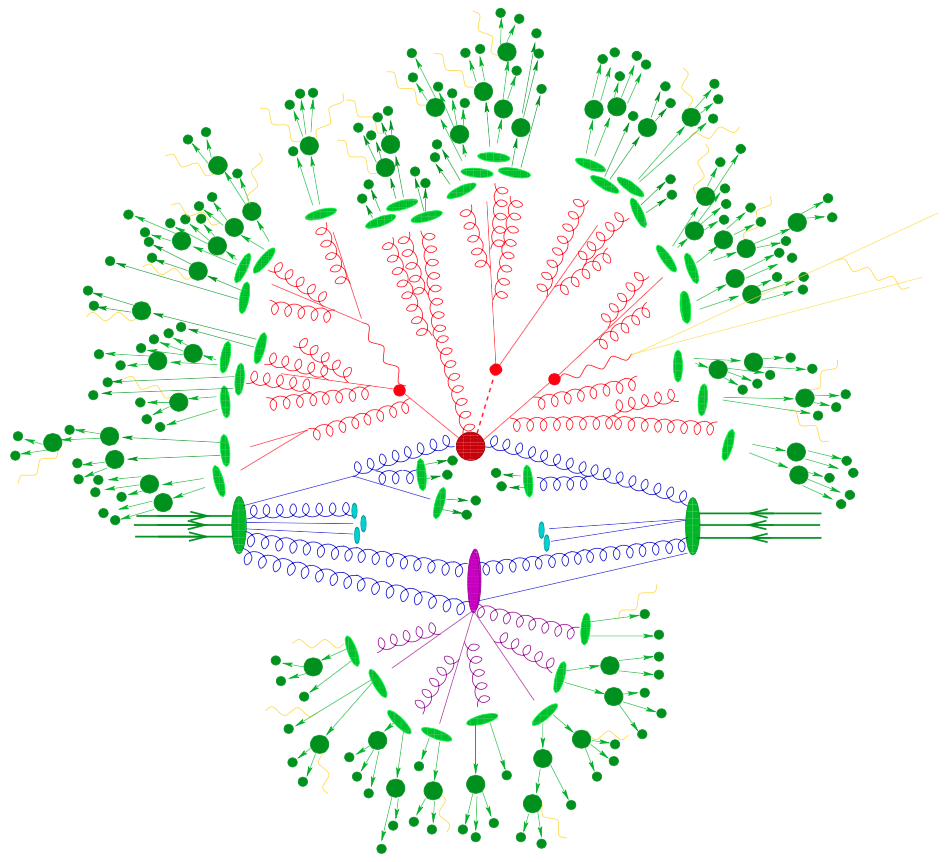
\includegraphics[width=0.95\textwidth]{\figpath/Chapter3/ttH_event.png}
    \caption{A graphical representation of a $t\bar{t}h$ event as seen by a MC event generator. The hard scatter interaction is represented by the red circle being produced by the two gluons coming of the incoming protons. The three small red dots represent the top quarks and the Higgs boson which then decay to additional hard QCD radiation. The underlying event is represented by the purple shapes and lines while the light green shapes are the final-state partons, which then hadronize and decay into the dark green circles. The yellow lines show the photon radiation which can occur at any state in the event generation process~\cite{Siegert:2010cru}.}
    \label{fig:ttH_event}
\end{figure}

Because protons are not elementary particles, it is important to discuss these interactions in terms of the partons inside the proton.
Hadrons, like the proton, are made up of valence quarks, sea quarks, and gluons\footnote{More precisely, protons are a bound state of two up quarks and a down quark.}.
In essence, the simulation of a proton-proton hard scatter interaction is the calculation of a cross section for an N-particle final state, seen in equation~\ref{eq:event_generation_cross_section}, where $a$ ($b$) is a parton carrying a fraction of the momentum $x_{a}$ ($x_{b}$) for hadron $A$ ($B$).
\begin{equation}
\label{eq:event_generation_cross_section}
\sigma_{N}^{AB}\left(s\right)=\int dx_{a}dx_{b}f_{a}\left(x_{a},\mu^{2}\right)f_{b}\left(x_{b},\mu^{2}\right)\hat{\sigma}_{N}^{ab}\left(\hat{s},\mu^{2}\right)
\end{equation}
The parton distribution function (PDF) of the form $f_{a,b}\left(x_{a,b},\mu^{2}\right)$ gives the probability density of finding such a parton with momentum fraction $x_{a,b}$ renormalized to scale $\mu^{2}$.
PDFs cannot be obtained using perturbative nor lattice QCD calculations.
Instead they are measured within the resolution of the existing experiments.
CMS makes use of the Martin-Stirling-Thorne-Watt (MSTW)~\cite{Martin:2009iq} and Coordinated Theoretical-Experimental Project on QCD (CTEQ) PDFs.
Fig.~\ref{fig:mstw} shows the NLO MSTW PDFs calculated for two different momentum scales.
Other terms include the center-of-mass energy of the interaction $\sqrt{\hat{s}}=\sqrt{x_{a}x_{b}s}$ where $\sqrt{s}$ is the center-of-mass energy of the proton-proton system and $\hat{\sigma}_{ab\rightarrow{X}}\left(\hat{s},\mu^{2}\right)$, which is the cross section for having a given set of initial state partons. The full form of the partonic cross section is given by 
\begin{equation}
\begin{split}\label{eq:event_generation_partonic_cross_section}
\hat{\sigma}_{N}^{ab}=\int_{cuts}d\hat{\sigma}_{N}^{ab}={}&\frac{\left(2\pi\right)^{4}S}{4\sqrt{\left(p_{1}{\cdot}p_{2}\right)^{2}-m_{1}^{2}m_{2}^{2}}}\times \\ &\int_{cuts} \left[\prod_{i=1}^{N}\frac{d^{3}q_{i}}{\left(2\pi\right)^{3}2E_{i}}\right]\delta^{4}\left(p_{1}+p_{2}-\sum_{i}^{N}q_{i}\right)|\mathcal{M}_{p_{1}p_{2}\rightarrow\{\vec{q}\}}^{ab}|^{2}
\end{split}
\end{equation}
where $p_{i}$ are the four-momenta of the incoming partons, $q_{i}$ and $E_{i}$ are the outgoing particle four-momenta and energies, $S$ is the product of $1/j!$ for j identical particles in the final state, and $\mathcal{M}_{p_{1}p_{2}\rightarrow\{\vec{q}\}}^{ab}$ is the ME associated to the kinematic configuration $p_{1}p_{2}\rightarrow\{\vec{q}\}$ with initial partons $a$ and $b$~\cite{Siegert:2010cru,Griffiths2008}.
In order to evaluate the parton level ME the event generator must either have the ME hard coded or it must be able to compute all of the Feynman diagrams associated with a given process.
A good example of this type of calculation can be found in Table 1.1 of~\cite{Siegert:2010cru}.
While the number of diagrams for a $2\rightarrow2$ or $2\rightarrow3$ process is limited and can be built and computed automatically, the problem becomes much more difficult for next to leading order (NLO) computations as the number of diagrams grows factorially~\cite{Kurihara:2002ne}.
The growth of the number of diagrams can be seen in fig.~\ref{fig:NumberOfDiagrams}.
In many cases the LO MEs and PDFs are used to generate events and a K-factor is used to scale the events to their NLO or NNLO predictions.
Besides computing the MEs, the the multi-dimensional phase space integration is quite complicated and requires the use of Monte-Carlo integration techniques~\cite{MonteCarloMethods}.

\begin{figure}[!hbt]
    \vspace*{-0.5cm}
    \centering
    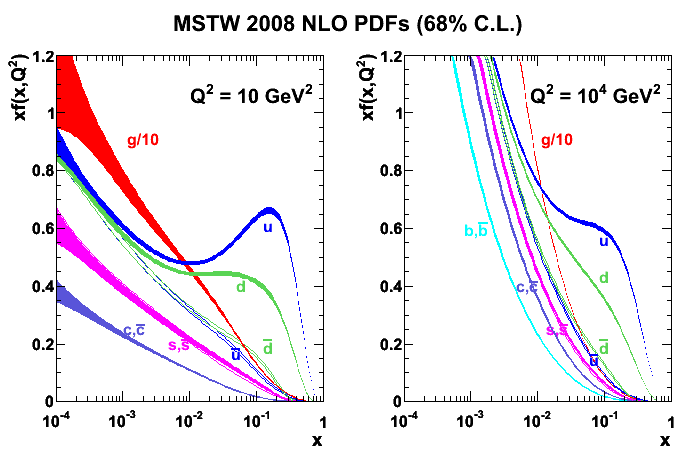
\includegraphics[width=0.95\textwidth]{\figpath/Chapter3/mstw2008nlo68cl_allpdfs.png}
    \caption{The MSTW PDFs calculated to NLO as a function of the momentum fraction for two different interaction momentum scales $Q^{2}$. In the case of synchrotron collisions $Q^{2}$ is the square of the total four-momentum of the proton-proton interaction. The right plot shows the momentum scale more commonly found at the LHC~\cite{Martin:2009iq}.}
    \label{fig:mstw}
\end{figure}

\begin{figure}[!hbt]
    \vspace*{-0.5cm}
    \centering
    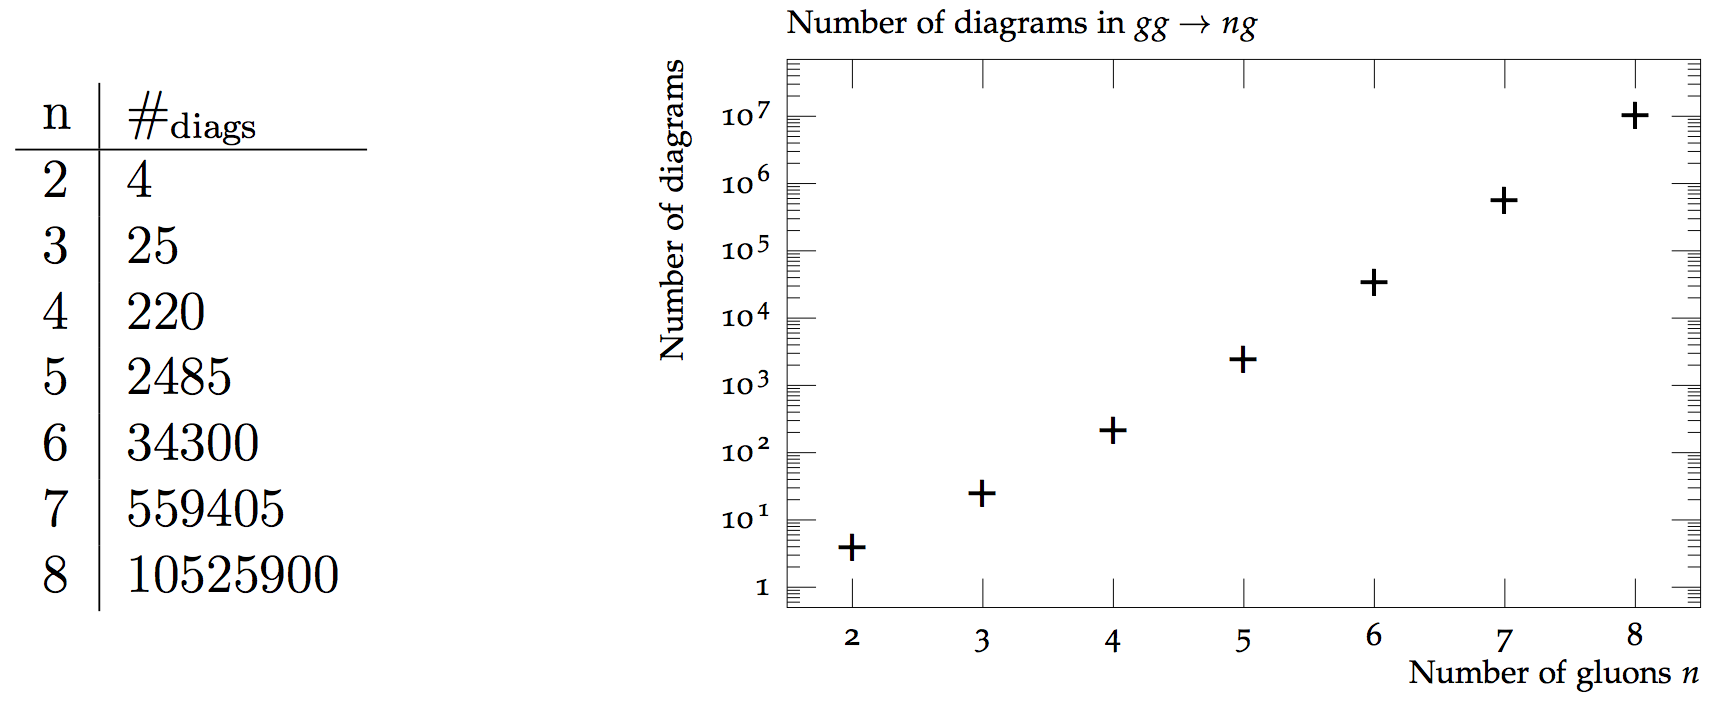
\includegraphics[width=0.95\textwidth]{\figpath/Chapter3/NumberOfDiagrams.png}
    \caption{The number of diagrams which must be calculated to fully calculate the $gg\rightarrow{ng}$ amplitude~\cite{Siegert:2010cru}.}
    \label{fig:NumberOfDiagrams}
\end{figure}

The parton shower takes the partons created by the hard process and UE and perturbatively evolves them down to the hadronization scale, at which point they form colorless hadrons.
The partons are initially produced at a scale $t'$ and the parton shower determines the scale $t<t'$ at which the parton should branch into two daughter particles, selecting the kinematics and flavors of those new particles.
This process continues recursively and only ceases once the hadronization scale is reached, $\mathcal{O}\left(\gev\right)$, where $\alpha_{s}$ becomes large and perturbative methods are no longer applicable. 
Generators make use of any number of phenomenological models, including the Lund string model~\cite{ANDERSSON198331,Andersson:1997hs} and the cluster hadronization model~\cite{WEBBER1984492,Winter:2003tt}, to turn this list of colored partons into colorless hadrons.
No matter the model used, the hadrons which result from these models are often unstable and will forced to decay into stable hadrons, which are defined to have a mean lifetime above a given threshold as defined by the experiment.

Various generators are used in this analysis, each with their own benefits and drawbacks. \textsc{pythia}~\cite{1126-6708-2006-05-026} is a general purpose event generator capable of handling many $2\rightarrow1,\text{ }2,\text{ }3$ processes.
It is capable of handling all of the needed generation steps including generating the hard scatter process, parton showering to the leading log (LL) level, hadronization, and the UE simulation. \textsc{pythia} makes use of the Lund string model for hadronization and describes the UE as additional, but not quite independent perturbative $2\rightarrow2$ scatterings. 
Another generator used is \textsc{Mad}\textsc{Graph}~\cite{Alwall:2014hca}, which more accurately simulates hard parton emission (i.e. ISR and FSR), but must be interfaced with \textsc{pythia} for showering soft and collinear radiation.
The \textsc{POWHEG}~\cite{Nason:2004rx,Alioli:2010xd} generator uses NLO matrix elements and PDFs and then matches this with a modified shower simulation.
Both \textsc{Mad}\textsc{Graph} and \textsc{POWHEG} are interfaced with \textsc{pythia} for hadronization.
For more accurate tau lepton decays CMS often uses the \textsc{tauola}~\cite{WAS200196} software package.

\section{Detector Simulation}
\label{sec:detector_simulation}

Event generation simulates the particle kinematics for a given event, but doesn't examine how the particles will interact with the detector and it's constituent materials or how the readout electronics will behave.
To simulate the response of the CMS detector, the generators are interfaced with a sophisticated detector simulation based on the \textsc{Geant4}~\cite{geant4nim,geant4ieee} software package, which takes into account the exact detector geometry as well as all materials used.
The alignment, calibration, and other conditions which may change over time are periodically checked and are stored in a database.
These conditions are used both for offline simulation and reconstruction as well as for online activities.
The final state particles from the event generator are sent to the detector simulation, which tracks the particles as they move through the detector depositing energy into what are called simulated hits (SimHits).
While the models of electromagnetic interactions are extremely precise, the hadronic interactions have a greater uncertainty associated with them.
The simulation goes through the data acquisition process, event simulating the responses of the photodetectors and readout electronics.
The resulting information is then analyzed by the same reconstruction process that the real data goes through and is stored using the ROOT~\cite{Brun199781} software library.